\documentclass{vldb}
\usepackage{graphicx}
\usepackage{caption}
\usepackage{subcaption}
%\usepackage{balance} 
\usepackage{epstopdf}
\usepackage{pbox}
\let\proof\relax
\let\endproof\relax
\usepackage{algorithm, algpseudocode, amsmath,amsthm,amssymb}

\graphicspath{ {./charts/}, {./exp/} }
\epstopdfsetup{outdir=./charts/}
\newcommand{\reminder}[1]{ {\mbox{$<==$}} [[[ { \bf #1 } ]]] {\mbox{$==>$}}}
\newtheorem{definition}{Definition}
\newtheorem{theorem}{Theorem}
\newtheorem{example}{Example}
\DeclareMathOperator*{\argmin}{argmin}
\DeclareMathOperator*{\argmax}{argmax}
\newcommand*{\argminl}{\argmin\limits}
\newcommand*{\argmaxl}{\argmax\limits}

\hyphenation{op-tical net-works semi-conduc-tor}

\begin{document}

% ****************** TITLE ****************************************

\title{A General and Parallel Platform for Mining Co-Movement Patterns over Large-scale Trajectories}

% ****************** AUTHORS **************************************

% You need the command \numberofauthors to handle the 'placement
% and alignment' of the authors beneath the title.
%
% For aesthetic reasons, we recommend 'three authors at a time'
% i.e. three 'name/affiliation blocks' be placed beneath the title.
%
% NOTE: You are NOT restricted in how many 'rows' of
% "name/affiliations" may appear. We just ask that you restrict
% the number of 'columns' to three.
%
% Because of the available 'opening page real-estate'
% we ask you to refrain from putting more than six authors
% (two rows with three columns) beneath the article title.
% More than six makes the first-page appear very cluttered indeed.
%
% Use the \alignauthor commands to handle the names
% and affiliations for an 'aesthetic maximum' of six authors.
% Add names, affiliations, addresses for
% the seventh etc. author(s) as the argument for the
% \additionalauthors command.
% These 'additional authors' will be output/set for you
% without further effort on your part as the last section in
% the body of your article BEFORE References or any Appendices.

%\author{
%	\IEEEauthorblockN{
%		Qi Fan\IEEEauthorrefmark{1},
%		Yuchen Li\IEEEauthorrefmark{1},
%		Dongxiang Zhang\IEEEauthorrefmark{2} and
%		Kian-Lee Tan\IEEEauthorrefmark{1}\IEEEauthorrefmark{2}
%		}
%	\IEEEauthorblockA{
%		\IEEEauthorrefmark{1}NUS Graduate School for Integrative Sciences and Engineering,
%		National University of Singapore, Singapore\\
%		\{fan.qi, liyuchen\}@nus.edu.sg
%	}
%	\IEEEauthorblockA{
%		\IEEEauthorrefmark{2}School of Computing,
%		National University of Singapore, Singapore \\
%		\{zhangdo,tankl\}@comp.nus.edu.sg
%	}
%}

\maketitle

\begin{abstract}

\end{abstract}


\section{Introduction}
The prevalence of positioning devices has drastically boosted 
the scale and spectrum of trajectory collection to an unprecedented level. 
Tremendous amounts of trajectories, in the form of sequenced spatial-temporal 
records, are continually generated from animal telemetry chips, 
vehicle GPSs and wearable devices. Data analysis on large-scale 
trajectories benefits a wide range of applications and services, 
including traffic planning~\cite{zheng2011urban}, animal analysis~\cite{li2010miningperiodic}, and social recommendations~\cite{bao2013survey}, to name just a few.


A crucial task of data analysis on top of trajectories is 
to discover co-moving patterns. A \emph{co-movement} pattern~\cite{li2013managing} 
refers to a group of objects traveling together for a certain period of time 
and the group is normally determined by spatial proximity. 
A pattern is prominent if the size of the group exceeds $M$ and the length of the duration exceeds $K$, where $M$ and $K$ are parameters specified by users. Rooted from such basic definition 
and driven by different mining applications, there are a bunch of variants 
of co-movement patterns that have been developed with more advanced constraints.

Table~\ref{tbl:existing_co_patterns} summarizes several popular co-moving pattern s 
with different constraints in the attributes of clustering in spatial proximity,
consecutiveness in temporal duration and computational complexity. 
In particular,  the \emph{flock}~\cite{gudmundsson2006flock} 
and the \emph{group}~\cite{wang2006grouppattern} patterns require 
all the objects in a group to be enclosed by a disk with radius $r$; 
whereas the \emph{convoy}~\cite{jeung2008convoy}, the \emph{swarm}~\cite{li2010swarm} 
and the \emph{platoon}~\cite{li2015platoon} patterns resort to density-based 
spatial clustering. 
In the temporal dimension, the \emph{flock}~\cite{gudmundsson2006flock} 
and the \emph{convoy}~\cite{jeung2008convoy} require all the timestamps 
of each detected spatial group to be consecutive, which is referred to as \emph{global consecutiveness}; 
whereas the \emph{swarm}~\cite{li2010swarm} does not impose any restriction. 
The \emph{group}~\cite{wang2006grouppattern} and the \emph{platoon}~\cite{li2015platoon} adopt a compromised manner by allowing
arbitrary gaps between the consecutive segments, which is called \emph{local consecutiveness}. 
They introduce a parameter $L$ to control the minimum length of each local consecutive segment.


\begin{table} \scriptsize
\centering
\begin{tabular}{|c|c|c|c|}
\hline 
 & {\tiny Proximity} & {\tiny Consecutiveness} & {\tiny Time Complexity}\\ 
\hline 
flock~\cite{gudmundsson2004flock} & disk-based &  global & $O(|\mathbb{O}||\mathbb{T}|(M + log(|\mathbb{O}|))$ \\ 
\hline 
convoy~\cite{jeung2008convoy} & density-based &   global & $O(|\mathbb{O}|^2+|\mathbb{O}||\mathbb{T}|)$\\ 
\hline 
swarm~\cite{li2010swarm} & density-based  & - & $O(2^{|\mathbb{O}|}|\mathbb{O}||\mathbb{T}|)$  \\ 
\hline 
group~\cite{wang2006grouppattern} & disk-based &  local & $O(|\mathbb{O}|^2|\mathbb{T}|)$ \\ 
\hline 
platoon~\cite{li2015platoon} & density-based &  local & $O(2^{|\mathbb{O}|}|\mathbb{O}||\mathbb{T}|)$\\ 
\hline 
\end{tabular} 
\caption{Constraints and complexity of co-movement patterns. The time complexity indicates the performance in the worst case, where $|\mathbb{O}|$ is the total number of objects and $|\mathbb{T}|$ is the number of descritized timestamps.}
\label{tbl:existing_co_patterns}
\end{table}




\begin{figure}[h]
\centering
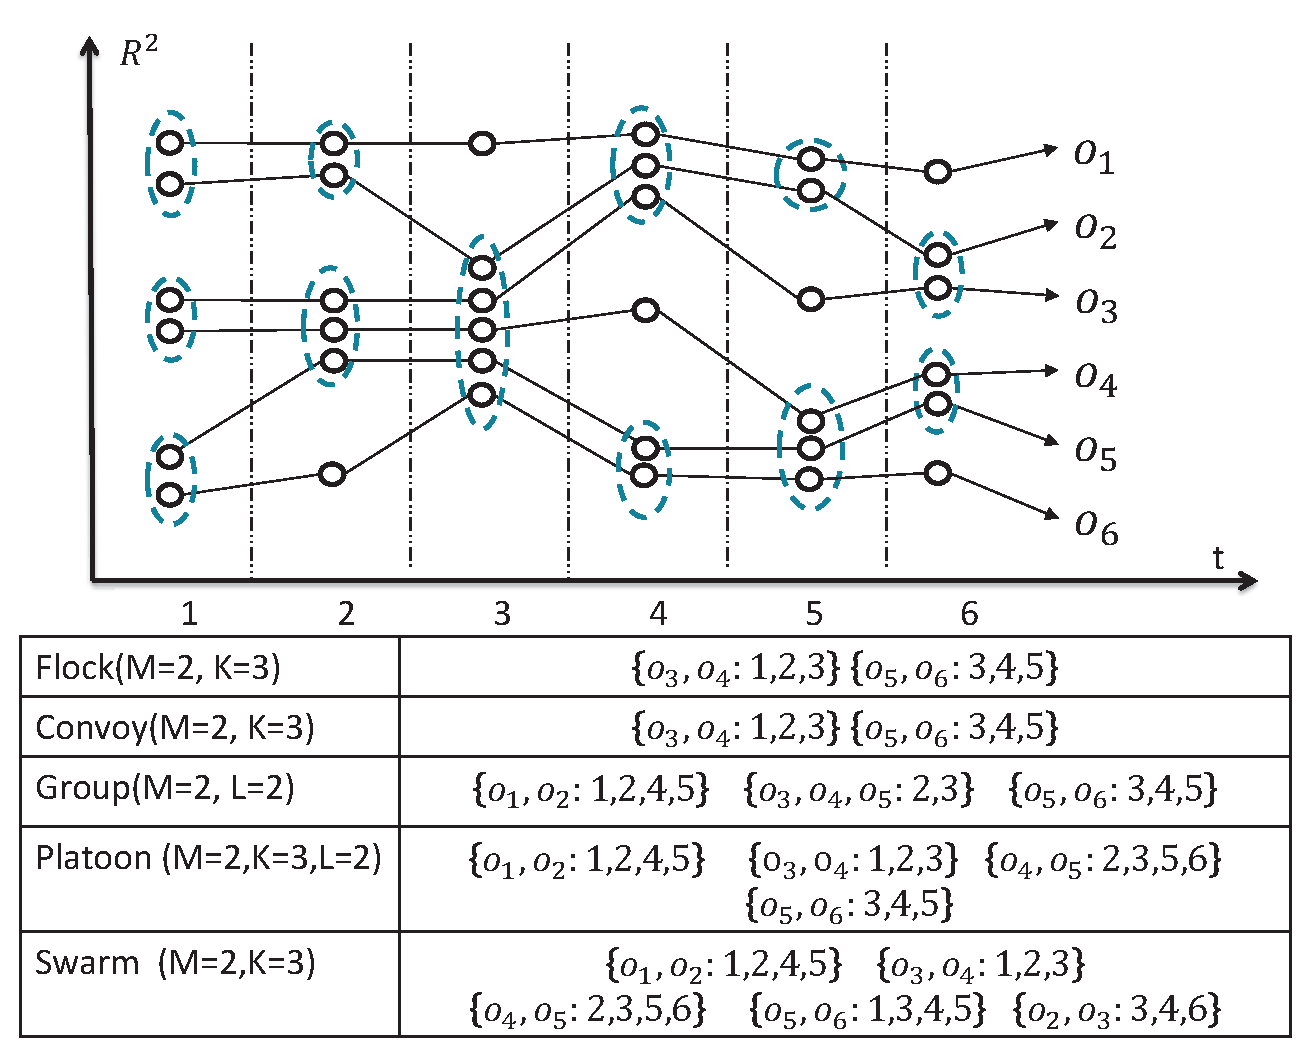
\includegraphics[width=0.45\textwidth]{related_work.eps}
\caption{Trajectories and co-movement patterns; The example consists of six trajectories across six snapshots. Objects in spatial clusters are enclosed by dotted circles. $M$ is the minimum cluster cardinality; $K$ denotes the minimum number of snapshots for the occurrence of a spatial cluster; and $L$ denotes the minimum length for local consecutiveness.}
\label{fig:related_work}
\end{figure}

Figure~\ref{fig:related_work} is an example to demonstrate the concepts of various co-movement patterns. The trajectory database consists of six moving objects and the temporal dimension is discretized into six snapshots. In each snapshot, we treat the clustering methods as a black-box and assume that they generate the same clusters. Objects in proximity are grouped in the dotted circles. As aforementioned, there are three parameters to determine the co-movement patterns and the default settings in this example are $M=2$, $K=3$ and $L=2$. Both the \emph{flock} and the \emph{convoy} require the spatial clusters to last for at least $K$ consecutive  timestamps. Hence,$\{o_3,o_4\}$ and $\{o_5,o_6\}$  remains the only two candidates matching the patterns. The \textit{swarm} relaxes the pattern matching by discarding the temporal consecutiveness constraint. Thus, it generates many more candidates than the \textit{flock} and the \textit{convoy}. The \textit{group} and the \textit{platoon} add another constraint on local consecutiveness to retain meaningful patterns. For instance, $\{o_1,o_2:1,2,4,5\}$ is a pattern matching local consecutiveness because timestamps $\{1,2\}$ and $\{4,5\}$ are two segments with length no smaller than $L=2$. The difference between the \textit{group} and the \textit{platoon} is that the \textit{platoon} has an additional parameter $K$ to specify the minimum number of snapshots for the spatial clusters. This explains why $\{o_3,o_4,o_5:2,3\}$ is a  \textit{group} pattern but not a \textit{platoon} pattern.

As can be seen, there are various co-movement patterns requested by different applications and it is cumbersome to design a tailored solution for each type. In addition, despite the generality of the \emph{platoon} (i.e., it can be reduced to other types of patterns via proper parameter settings), it suffers from the so-called \emph{loose-connection} anomaly. We use two objects $o_1$ and $o_2$ in Figure~\ref{fig:platoon_weakpoint} as an example to illustrate the scenario. These two objects form a \emph{platoon} pattern in timestamps $\{1,2,3,102,103,104\}$. However, the two consecutive segments are $98$ timestamps apart, resulting in a false positive co-movement pattern. In reality, such an anomaly may be caused  by the periodic movements of unrelated objects, such as vehicles stopping at the same petrol station or animals pausing at the same water source. 
Unfortunately, none of the existing patterns have directly addressed this anomaly.


%As can be seen, there are various co-movement patterns requested by different 
%applications and it is cumbersome to design a tailored solution for each type. 
%As pointed in \cite{li2015platoon, li2010swarm}, stringent temporal constraints (e.g., global consecutiveness on \emph{flock} and \emph{convoy}) may miss out many interesting patterns. However, we 
%further observe that pattern definitions with overly-relaxed temporal constraints (e.g., \emph{swarm}, \emph{group} and \emph{platoon}) lose the fine control of a pattern which lead to noisy results and unnecessary computations. We name this scenario as \emph{loose-connection} anomaly. To illustrate, as shown in Figure~\ref{fig:platoon_weakpoint}, the two objects $o_1, o_2$ form a \emph{platoon} pattern 
%$\{o_1,o_2:1,2,3,102,103,104\}$. However, the consecutive segments are $98$ timestamps apart, 
%making the co-moving behavior very loose.
%In reality, such an anomaly is likely induced by the periodic movements of unrelated objects 
%such as, vehicles stopping at the same petrol station, animals pausing at the same water source etc.  Interestingly, none of the temporal-relaxed patterns (e.g., \emph{swarm}, \emph{group} and \emph{platoon}) are able to directly avoid such an anomaly.

%In addition, existing pattern definitions are not expressive enough and may miss 
%interesting patterns or return noisy results. We summarize 
%the two scenarios as \emph{missing-pattern} anomaly
%and \emph{loose-connection} anomaly.
%A \emph{missing-pattern} anomaly arises due to the stringent constraints on the pattern duration.
%As shown in Figure~\ref{fig:platoon_weakpoint} (a), if we set $K=4$, 
%neither \emph{flock}s nor \emph{convoy}s can be discovered. This is because
%$o_1$ is away from $o_2$ at timestamp $4$, which is likely caused by
%the traffic control or the clustering inaccuracy at time $4$. On the other hand,
%the \emph{loose-connection} anomaly occurs due to an over-relaxed constraint on 
%the duration. As shown in Figure~\ref{fig:platoon_weakpoint} (b),
%the two objects $o_1, o_2$ form a \emph{platoon} pattern 
%$\{o_1,o_2:1,2,3,102,103,104\}$. However, the consecutive segments are $98$ timestamps apart, 
%making the co-moving behavior very weak.
%In reality, such an anomaly is likely to be induced by the periodic movements of unrelated objects 
%such as, vehicles stopping at the same petrol station, animals pausing at the same water source etc. 
%It is easy to see that none of the existing co-movement patterns are able to avoid these two anomalies.

\begin{figure}[h]
\center
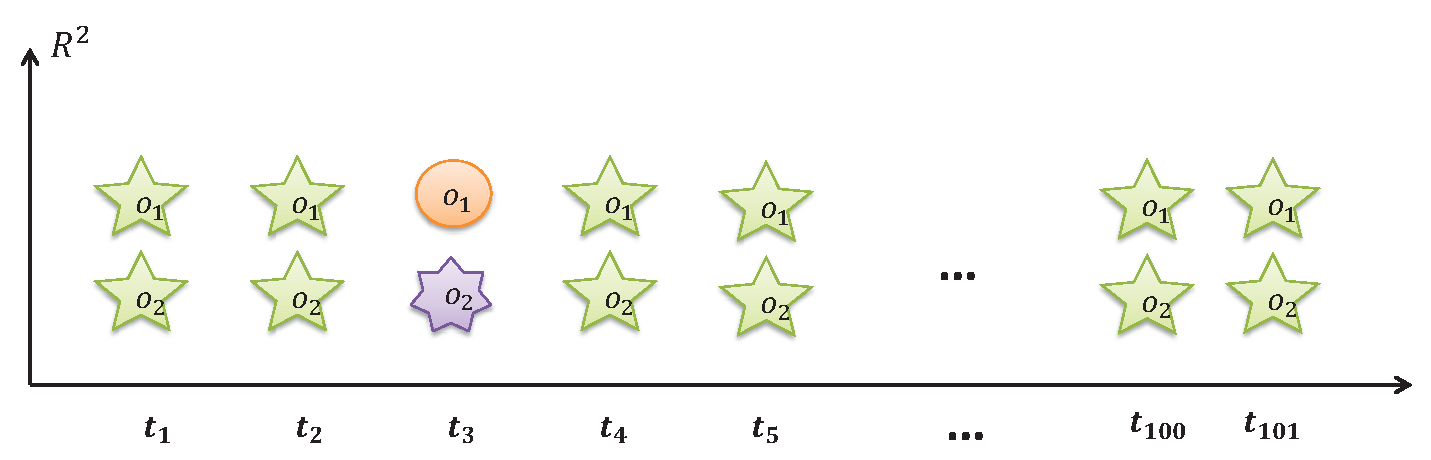
\includegraphics[width=0.33\textwidth]{platoon_weakpoint.eps}
\caption{\emph{Loose-connection} anomaly. Even though $\{o_1, o_2: 1,2,3,102,103,104\}$ is considered as a valid \emph{platoon} pattern, it is highly probable that these two objects are not related as the two consecutive segments  are 98 timestamps apart. 
}
\label{fig:platoon_weakpoint}
\end{figure}

%In current literature,
%users are unable to explicitly exclude the loosely-connected patterns even when those patterns are unwanted.
%
%
% we summarize two anomalies 
%The \emph{missing-pattern}~\cite{li2010swarm} anomaly arises due to the stringent constraints on the duration of a pattern. As shown in 
%Figure~\ref{fig:platoon_weakpoint} (a).  As we notice, object $o_1$ is temporally far from $o_2$ at timestamp $4$, which is likely to be
%the result of errors in interpretation of missing points, or $o_1$ faces traffic control at time $4$. Such an anomaly can
%be resolved by \emph{swarm} and \emph{platoon} due to a relaxed constraint on the duration. However, 
%\emph{swarm} and \emph{platoon}'s relaxations encompass a type of non-interesting patterns which is referred
%as \emph{loose-connection}~\cite{li2015platoon} anomaly. 
%
%
%%This is because that \emph{platoon} allows the timestamps in a pattern duration to be in arbitrary distance, making the object group loosely
%connected. For instance, patterns with duration $\{1,2,100,101\}$ could be a valid \emph{platoon}; however, the two timestamps $2,100$ are too far from each other.

%For instance, PUT THE FIGURE AND EXPLANATION HERE.

%\begin{figure}[h]
%\center
%\includegraphics[width=0.35\textwidth]{rw_perf_O.eps}
%\caption{Two anomalies in existing patterns. (a) \emph{Missing-pattern} anomaly
%in \emph{flock} and \emph{convoy}. When $K=4$, none of the two patterns can be discovered. (b) \emph{Loose-connection} anomaly in \emph{platoon} and \emph{swarm}. The consecutive segment of $o_1$ and $o_2$ are 98 timestamps apart, however, the pattern $\{o_1, o_2: 1,2,3,102,103,104\}$ is included in platoon and swarm results.}
%\label{fig:platoon_weakpoint}
%\end{figure}


The other issue with existing methods is that they are built on top of centralized indexes which may not be scalable. Table~\ref{tbl:existing_co_patterns} shows their theoretical complexities in the worst cases and the largest real dataset ever evaluated in previous studies is up to million-scale points collected from hundreds of moving objects. In practice, the dataset is of much higher scale and the scalability of existing methods is left unknown. Thus, we conduct an experimental evaluation with $4000$ objects moving for $2500$ timestamps to examine the scalability. Results in Figures~\ref{fig:related_work_scalability} show that their performances degrade dramatically as 
the dataset scales up. For instance,
the detection time of \emph{swarm} drops fifteen times as the number of objects grows from \emph{1k} to \emph{4k}. Similarly,
the performance of \emph{group} drops near fourteen times as the number of snapshots grows from \emph{1k} to \emph{2.5k}.
These observations imply that existing methods are not scalable to support large-scale trajectory databases. 

%It is easy to spot that none of the existing solutions are scalable to handle large-scale trajectories which include near billions of data points.
%In fact, as shown in Table~, the mining of co-movement patterns require high complexity. For instance, the
%complexities of \emph{swarm} and \emph{platoon} are already exponential. 
%Therefore, none of them can handle millions of trajectories efficiently. 
%CAN YOU ANALYSE THEIR COMPLEXITY TO ADDRESS THE PROBLEM OF SCALABILITY.
\begin{figure}[h]
    \centering
    \begin{subfigure}[b]{0.23\textwidth}
            \centering
            \includegraphics[width=\textwidth]{rw_perf_O.eps}
		\subcaption{Vary objects $|\mathbb{T}| = 1k$}
    \label{fig:fig1}
    \end{subfigure}
    \begin{subfigure}[b]{0.23\textwidth}
            \centering
            \includegraphics[width=\textwidth]{rw_perf_T.eps}
         \subcaption{Vary timestamps $|\mathbb{O}| = 1k$}
    \label{fig:fig2}
    \end{subfigure}
    \caption{Performance measures on existing co-movement patterns. A sampled Geolife dataset
    is used with up two 4 million data points. Pattern parameters are $M=20,K=100,L=20$.}
    \label{fig:related_work_scalability}
\end{figure}




Therefore, our primary contributions in this paper are to close these two gaps. 
First, we propose the \emph{general co-movement pattern} (GCMP) which models
various co-moment patterns in a unified way and can avoid 
the \emph{loose-connection} anomaly. In GCMP, we introduce a new gap parameter $G$ to pose a constraint on the temporal gap between two consecutive segments. By setting a feasible $G$, the loose-connection anomaly can be avoided. In addition, our GCMP is both general and expressive. It can be reduced to any of the previous patterns by customizing the parameters.

%Therefore, users are 
%still able to exclude non-consecutive patterns 
%or include loosely-connected patterns when they feel necessary.


%We introduce the gap parameter $G$,
%When such loosely-connected patterns are unwanted, users currently are unable to directly control the outputs.
%To cope with both of the two anomalies, we propose 
%by introducing the gap parameter $G$, 

%By so doing, we gain a fine-grained control s, which As we show in later sections, the general co-movement pattern is able to express existing patterns by setting appropriate parameters. 
%IS IT POSSIBLE TO USE FIGURE 1 TO ADDRESS THE PROBLEM OF PLATOON, INSTEAD OF PROPOSING A NEW EXAMPLE SCENARIO?
%

Second, we investigate deploying our GCMP detector on MapReduce platforms (such as Hadoop and Spark) to tackle the scalability issue. Our technical contributions are three-fold. First, we replicate the snapshots in multiple data chunks to support efficient parallel processing. Second, we devise a novel \emph{Star Partition and Mining} (SPM) algorithm as a fine-granularity partitioning strategy to achieve workload balance. For each star, an Apriori method is adopted to mine the co-movement patterns. Third, we propose two types of optimization techniques to further improve the performance, including \emph{edge-simplification} to boost the shuffle process and \emph{temporal monotonicity pruning} and 
\emph{forward closure checking} to significantly reduce the number of enumerated candidates in the Apriori algorithm.



%
%Second, we investigate on deploying our GCMP detector to facilitate scalable pattern mining.
%In order to support large real trajectories, to the best of our knowledge, we
%are the first to study GCMP mining in MapReduce (MR) systems. There are a
%few challengers associated with designing an efficient MR-based pattern 
%detection algorithms. 
%
%First, in order to support effective parallelism, we need
%to partition the trajectory database with almost equal sizes. Our initial attempts
%develops a temporal based partition approached named as 
%\emph{Temporal Replication and Mining} (TRM). In TRM, neighboring snapshots form
%a equal-sized partition such that co-movement patterns can be mined independently.
%However, such a scheme require $O(|\mathbb{T}|)$ replication of input, which is 
%inefficient for large-scale trajectories. To support efficient mining, 
%we design a novel \emph{Star Partition and Mining} (SPM) approach which utilize
%the potential co-movement relationship among objects.
%
%Our initial attempt develops a naive but effective 
%\emph{Temporal Replication and Mining} (TRM) approach 
%which requires to replicate entire data set $O(|\mathbb{T}|)$ times. Such a 
%large set of 

%There
%are a few challenges arises in designing the MR based pattern detection algorithm.
%First, we 

%The major challenge
%we face is to make proper data partitions such
%that each partition can be efficiently processed independently. Our initial attempt develops
%a naive but effective \emph{Temporal Replication and Mining} (TRM) approach which requires to replicate
%entire data set $O(|\mathbb{T}|)$ times. To improve the efficiency, we design a novel \emph{Star Partition and Mining} (SPM)
%algorithm. In SPM, potential co-moving objects are first grouped into partitions. Subsequently,
%an apriori based method is applied to discover the patterns from each partition.
%Despite the simpleness of the star partition, we theoretically prove its correctness
%and optimality. Using SPM as the foundation, we develop and integrate
%a series of optimization techniques including \emph{edge simplification}, \emph{candidate pruning}
%and \emph{forward closure checking} to further boost the
%performances.
%


%
%Second, we investigate how to deploy our GCMP detector  on Spark for scalable pattern mining.
%The major challenge in designing MapReduce-based algorithms is to make proper partitions of input data.
%In GCMP mining, we enforce both the \emph{soundness} and the \emph{completeness} 
%of the partitions. Such properties ensure that neither false-patterns 
%nor miss-patterns are possible in our solution. To meet such partition requirements
%as well as to keep the shuffle amount to a minimum, 
%we first design a naive \emph{Temporal Replication and Mining} (TRM)
%approach, which partitions trajectories into groups of consecutive snapshots. Then, we design a line-sweep
%method for mining GCMP from each partition. We prove that in TRM, the partition is complete and sound when a snapshot is replicated $O(|T|)$ times. 
%Then, we design a novel \emph{Star Partition and Mining} (SRM) approach which significantly reduces the data shuffled
%as compare to TRM. In SRM, we design a conceptual connection graph based on proximity among objects. We adapt
%a \emph{star partition} which cut the graph by replicating vertices. Afterwards, we design an Apriori-like method to mine
%GCMP in each partition. We prove the correctness of SPM and show that total data been replicated is $O(|\mathbb{O}|)$. 
%Despite the simpleness of star partition, we theoretically prove its optimality.
%Furthermore, we utilize \emph{temporal monotonicity} to further reduce the 
%shuffling and mining cost in SPM. 
%Lastly, we adapt various engineering level techniques to support efficiently deploying our algorithms in 
%Apache Spark which is one of the most popular MapReduce platforms.

%we design a novel star-based partition scheme to efficiently partition objects based on their
%belonging clusters. Based on the star partition, we then propose a series of optimization techniques which
%largely improve the system performance. NEED TO EMPHASIZE YOUR TECHNICAL CONTRIBUTION!

We conduct a set of extensive experiments on XXX datasets with billion-scale trajectory points. The results show that XXX.

The rest of our paper is organized as follows: Section~\ref{sec:related_works} summarizes the relevant literature on 
trajectory pattern mining; Section~\ref{sec:definition} forms the definition of the general co-movement pattern mining; Section~\ref{sec:system_overview} presents our parallel architecture; The solution of mining the general co-movement pattern mining is presented in Section~\ref{sec:trm_solution} and Section~\ref{sec:spm_solution}. Section~\ref{sec:optimization} discusses various optimization techniques to boost the system performance; Section~\ref{sec:experiment} conducts extensive experiments to showcase the usefulness and efficiency of our system and finally Section~\ref{sec:conclusion} concludes our paper.




%\section{Introduction}
The prevalence of positioning devices has drastically boosted 
the scale and spectrum of trajectory collection to an unprecedented level. 
Tremendous amounts of trajectories, in the form of sequenced spatial-temporal 
records, are continually generated from animal telemetry chips, 
vehicle GPSs and wearable devices. Data analysis on large-scale 
trajectories benefits a wide range of applications and services, 
including traffic planning~\cite{zheng2011urban}, animal analysis~\cite{li2010miningperiodic}, and social recommendations~\cite{bao2013survey}, to name just a few.


A crucial task of data analysis on top of trajectories is 
to discover co-moving patterns. A \emph{co-movement} pattern~\cite{li2013managing} 
refers to a group of objects traveling together for a certain period of time 
and the group is normally determined by spatial proximity. 
A pattern is prominent if the size of the group exceeds $M$ and the length of the duration exceeds $K$, where $M$ and $K$ are parameters specified by users. Rooted from such basic definition 
and driven by different mining applications, there are a bunch of variants 
of co-movement patterns that have been developed with more advanced constraints.

Table~\ref{tbl:existing_co_patterns} summarizes several popular co-moving pattern s 
with different constraints in the attributes of clustering in spatial proximity,
consecutiveness in temporal duration and computational complexity. 
In particular,  the \emph{flock}~\cite{gudmundsson2006flock} 
and the \emph{group}~\cite{wang2006grouppattern} patterns require 
all the objects in a group to be enclosed by a disk with radius $r$; 
whereas the \emph{convoy}~\cite{jeung2008convoy}, the \emph{swarm}~\cite{li2010swarm} 
and the \emph{platoon}~\cite{li2015platoon} patterns resort to density-based 
spatial clustering. 
In the temporal dimension, the \emph{flock}~\cite{gudmundsson2006flock} 
and the \emph{convoy}~\cite{jeung2008convoy} require all the timestamps 
of each detected spatial group to be consecutive, which is referred to as \emph{global consecutiveness}; 
whereas the \emph{swarm}~\cite{li2010swarm} does not impose any restriction. 
The \emph{group}~\cite{wang2006grouppattern} and the \emph{platoon}~\cite{li2015platoon} adopt a compromised manner by allowing
arbitrary gaps between the consecutive segments, which is called \emph{local consecutiveness}. 
They introduce a parameter $L$ to control the minimum length of each local consecutive segment.


\begin{table} \scriptsize
\centering
\begin{tabular}{|c|c|c|c|}
\hline 
 & {\tiny Proximity} & {\tiny Consecutiveness} & {\tiny Time Complexity}\\ 
\hline 
flock~\cite{gudmundsson2004flock} & disk-based &  global & $O(|\mathbb{O}||\mathbb{T}|(M + log(|\mathbb{O}|))$ \\ 
\hline 
convoy~\cite{jeung2008convoy} & density-based &   global & $O(|\mathbb{O}|^2+|\mathbb{O}||\mathbb{T}|)$\\ 
\hline 
swarm~\cite{li2010swarm} & density-based  & - & $O(2^{|\mathbb{O}|}|\mathbb{O}||\mathbb{T}|)$  \\ 
\hline 
group~\cite{wang2006grouppattern} & disk-based &  local & $O(|\mathbb{O}|^2|\mathbb{T}|)$ \\ 
\hline 
platoon~\cite{li2015platoon} & density-based &  local & $O(2^{|\mathbb{O}|}|\mathbb{O}||\mathbb{T}|)$\\ 
\hline 
\end{tabular} 
\caption{Constraints and complexity of co-movement patterns. The time complexity indicates the performance in the worst case, where $|\mathbb{O}|$ is the total number of objects and $|\mathbb{T}|$ is the number of descritized timestamps.}
\label{tbl:existing_co_patterns}
\end{table}




\begin{figure}[h]
\centering
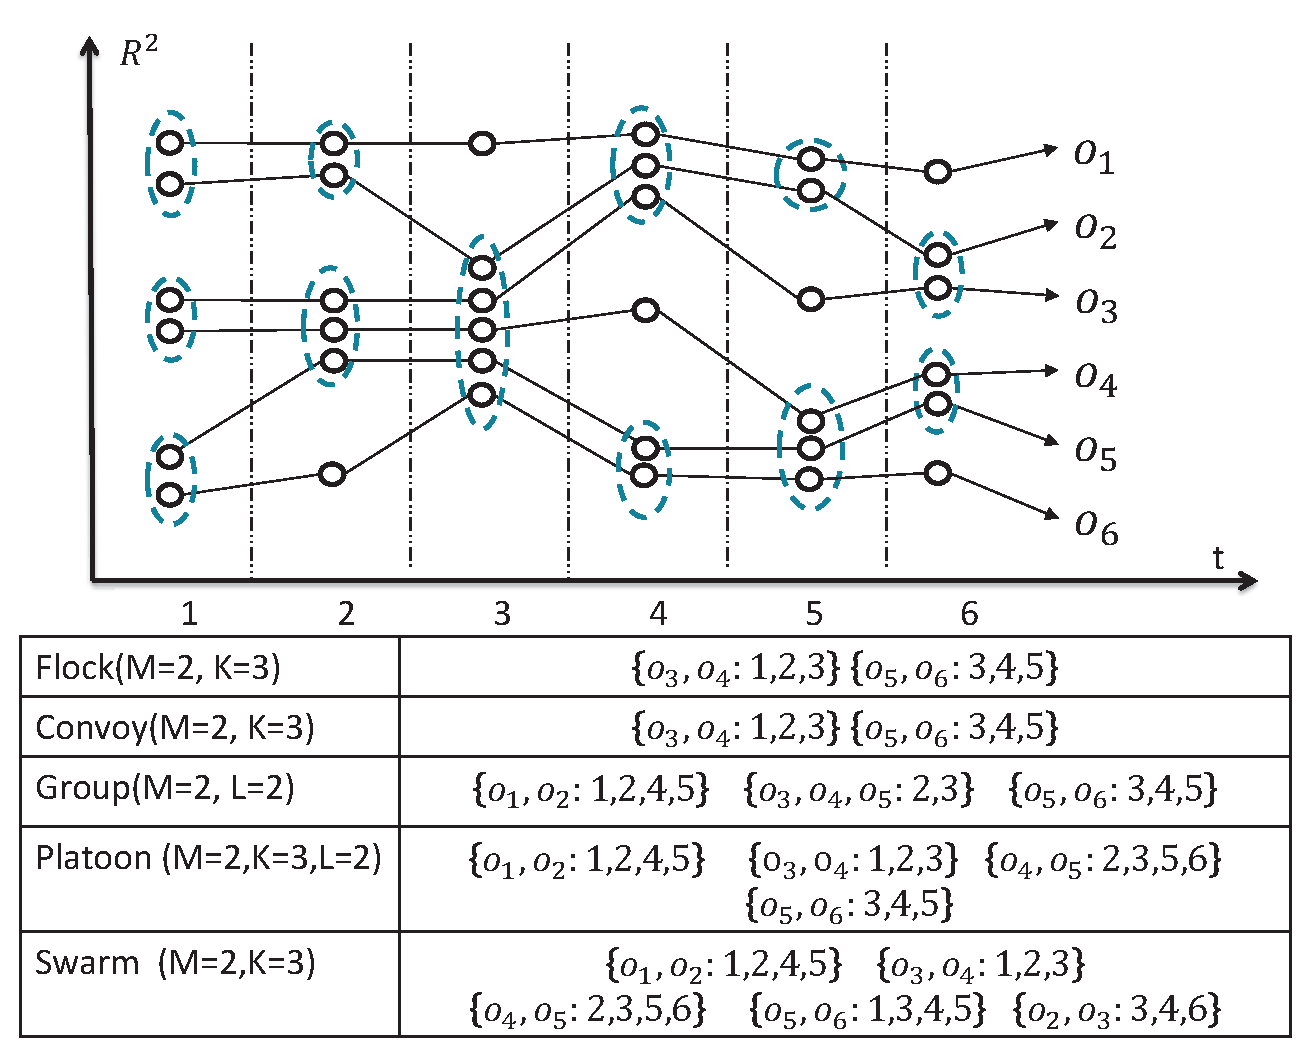
\includegraphics[width=0.45\textwidth]{related_work.eps}
\caption{Trajectories and co-movement patterns; The example consists of six trajectories across six snapshots. Objects in spatial clusters are enclosed by dotted circles. $M$ is the minimum cluster cardinality; $K$ denotes the minimum number of snapshots for the occurrence of a spatial cluster; and $L$ denotes the minimum length for local consecutiveness.}
\label{fig:related_work}
\end{figure}

Figure~\ref{fig:related_work} is an example to demonstrate the concepts of various co-movement patterns. The trajectory database consists of six moving objects and the temporal dimension is discretized into six snapshots. In each snapshot, we treat the clustering methods as a black-box and assume that they generate the same clusters. Objects in proximity are grouped in the dotted circles. As aforementioned, there are three parameters to determine the co-movement patterns and the default settings in this example are $M=2$, $K=3$ and $L=2$. Both the \emph{flock} and the \emph{convoy} require the spatial clusters to last for at least $K$ consecutive  timestamps. Hence,$\{o_3,o_4\}$ and $\{o_5,o_6\}$  remains the only two candidates matching the patterns. The \textit{swarm} relaxes the pattern matching by discarding the temporal consecutiveness constraint. Thus, it generates many more candidates than the \textit{flock} and the \textit{convoy}. The \textit{group} and the \textit{platoon} add another constraint on local consecutiveness to retain meaningful patterns. For instance, $\{o_1,o_2:1,2,4,5\}$ is a pattern matching local consecutiveness because timestamps $\{1,2\}$ and $\{4,5\}$ are two segments with length no smaller than $L=2$. The difference between the \textit{group} and the \textit{platoon} is that the \textit{platoon} has an additional parameter $K$ to specify the minimum number of snapshots for the spatial clusters. This explains why $\{o_3,o_4,o_5:2,3\}$ is a  \textit{group} pattern but not a \textit{platoon} pattern.

As can be seen, there are various co-movement patterns requested by different 
applications and it is cumbersome to design a tailored solution for each type. 
As pointed in \cite{li2015platoon, li2010swarm}, stringent temporal constraints (e.g., global consecutiveness on \emph{flock} and \emph{convoy}) may miss out many interesting patterns. However, we observe that pattern definitions with overly-relaxed temporal constraints (e.g., \emph{swarm}, \emph{group} and \emph{platoon}) lose the fine control of a pattern which introduce noisy results and unnecessary computations. We name this scenario as \emph{loose-connection} anomaly. To illustrate, as shown in Figure~\ref{fig:platoon_weakpoint}, the two objects $o_1, o_2$ form a \emph{platoon} pattern 
$\{o_1,o_2:1,2,3,102,103,104\}$. However, the consecutive segments are $98$ timestamps apart, 
making the co-moving behavior very loose.
In reality, such an anomaly is likely induced by the periodic movements of unrelated objects 
such as, vehicles stopping at the same petrol station, animals pausing at the same water source etc.  Interestingly, none of the temporal-relaxed patterns (e.g., \emph{swarm}, \emph{group} and \emph{platoon}) is able to avoid such an anomaly directly.

%In addition, existing pattern definitions are not expressive enough and may miss 
%interesting patterns or return noisy results. We summarize 
%the two scenarios as \emph{missing-pattern} anomaly
%and \emph{loose-connection} anomaly.
%A \emph{missing-pattern} anomaly arises due to the stringent constraints on the pattern duration.
%As shown in Figure~\ref{fig:platoon_weakpoint} (a), if we set $K=4$, 
%neither \emph{flock}s nor \emph{convoy}s can be discovered. This is because
%$o_1$ is away from $o_2$ at timestamp $4$, which is likely caused by
%the traffic control or the clustering inaccuracy at time $4$. On the other hand,
%the \emph{loose-connection} anomaly occurs due to an over-relaxed constraint on 
%the duration. As shown in Figure~\ref{fig:platoon_weakpoint} (b),
%the two objects $o_1, o_2$ form a \emph{platoon} pattern 
%$\{o_1,o_2:1,2,3,102,103,104\}$. However, the consecutive segments are $98$ timestamps apart, 
%making the co-moving behavior very weak.
%In reality, such an anomaly is likely to be induced by the periodic movements of unrelated objects 
%such as, vehicles stopping at the same petrol station, animals pausing at the same water source etc. 
%It is easy to see that none of the existing co-movement patterns are able to avoid these two anomalies.

\begin{figure}[h]
\center
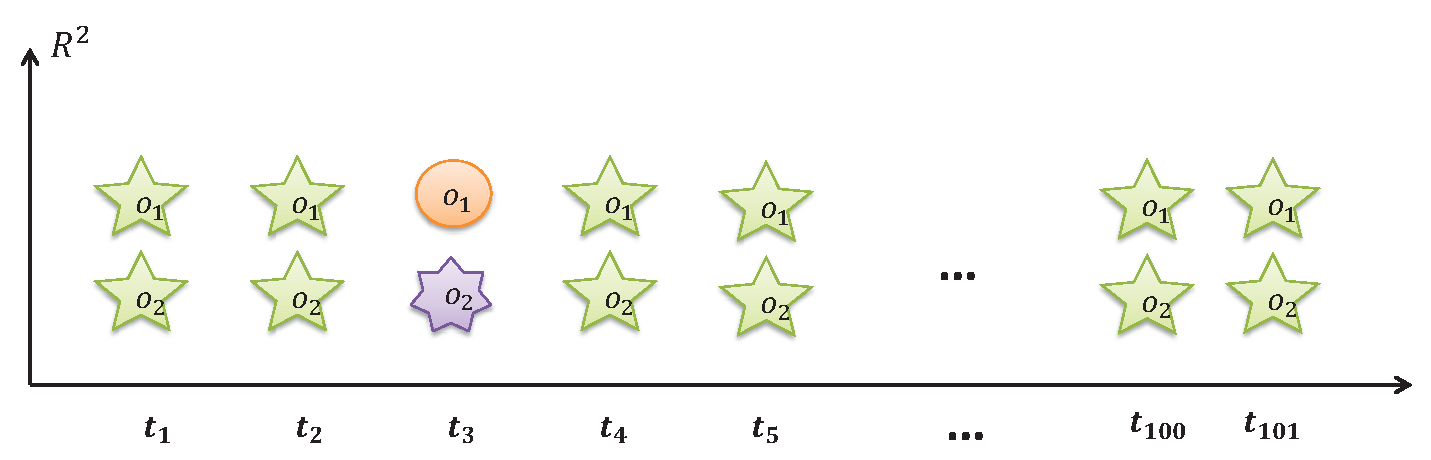
\includegraphics[width=0.35\textwidth]{platoon_weakpoint.eps}
\caption{\emph{Loose-connection} anomaly. The consecutive segment of $o_1$ and $o_2$ are 98 timestamps apart, however, the pattern $\{o_1, o_2: 1,2,3,102,103,104\}$ is included in \emph{platoon}, \emph{swarm} and \emph{group} results.}
\label{fig:platoon_weakpoint}
\end{figure}

%In current literature,
%users are unable to explicitly exclude the loosely-connected patterns even when those patterns are unwanted.
%
%
% we summarize two anomalies 
%The \emph{missing-pattern}~\cite{li2010swarm} anomaly arises due to the stringent constraints on the duration of a pattern. As shown in 
%Figure~\ref{fig:platoon_weakpoint} (a).  As we notice, object $o_1$ is temporally far from $o_2$ at timestamp $4$, which is likely to be
%the result of errors in interpretation of missing points, or $o_1$ faces traffic control at time $4$. Such an anomaly can
%be resolved by \emph{swarm} and \emph{platoon} due to a relaxed constraint on the duration. However, 
%\emph{swarm} and \emph{platoon}'s relaxations encompass a type of non-interesting patterns which is referred
%as \emph{loose-connection}~\cite{li2015platoon} anomaly. 
%
%
%%This is because that \emph{platoon} allows the timestamps in a pattern duration to be in arbitrary distance, making the object group loosely
%connected. For instance, patterns with duration $\{1,2,100,101\}$ could be a valid \emph{platoon}; however, the two timestamps $2,100$ are too far from each other.

%For instance, PUT THE FIGURE AND EXPLANATION HERE.

%\begin{figure}[h]
%\center
%\includegraphics[width=0.35\textwidth]{rw_perf_O.eps}
%\caption{Two anomalies in existing patterns. (a) \emph{Missing-pattern} anomaly
%in \emph{flock} and \emph{convoy}. When $K=4$, none of the two patterns can be discovered. (b) \emph{Loose-connection} anomaly in \emph{platoon} and \emph{swarm}. The consecutive segment of $o_1$ and $o_2$ are 98 timestamps apart, however, the pattern $\{o_1, o_2: 1,2,3,102,103,104\}$ is included in platoon and swarm results.}
%\label{fig:platoon_weakpoint}
%\end{figure}


The other issue with existing methods is that they are 
built on top of centralized indexes that are not scalable. 
To the best of our knowledge, the maximum number of trajectories 
ever evaluated is up to hundreds of trajectories. 
In practice, it is rather common to collect at least hundreds of thousands of trajectories 
and their scalability is left unknown. We conduct a theoretical analysis on the worst-case complexity (as listed in Table~\ref{tbl:existing_co_patterns}) as well as an experimental evaluation with a real trajectory database including million-scale points(as shown in Figure~\ref{fig:related_work_scalability}). 
Results show that their performances degrade dramatically as the dataset size scales up. For instances,
performance of \emph{swarm} drops five times as the number of objects grows from \emph{1k} to \emph{2k}. Similarly,
performance of \emph{group} drops over seven times as the number of snapshots grows from \emph{1.5k} to \emph{2.4k}.
It is easy to spot that none of the existing solutions are scalable to handle large-scale trajectories which may include billion-scale points.
%In fact, as shown in Table~, the mining of co-movement patterns require high complexity. For instance, the
%complexities of \emph{swarm} and \emph{platoon} are already exponential. 
%Therefore, none of them can handle millions of trajectories efficiently. 
%CAN YOU ANALYSE THEIR COMPLEXITY TO ADDRESS THE PROBLEM OF SCALABILITY.
\begin{figure}[h]
    \centering
    \begin{subfigure}[b]{0.23\textwidth}
            \centering
            \includegraphics[width=\textwidth]{rw_perf_O.eps}
		\subcaption{$1k$ objects}
    \label{fig:fig1}
    \end{subfigure}
    \begin{subfigure}[b]{0.23\textwidth}
            \centering
            \includegraphics[width=\textwidth]{rw_perf_T.eps}
         \subcaption{$1.2k$ timestamps}
    \label{fig:fig2}
    \end{subfigure}
    \caption{Performance measures on existing co-movement patterns. A sampled Geolife data set
    is used with over 2 million points.}
    \label{fig:related_work_scalability}
\end{figure}




Therefore, our primary contributions in this paper are to close these two gaps. 
First, we propose the \emph{general co-movement pattern} (GCMP) which models
various co-moment patterns in a unified way while avoids 
the \emph{loose-connection} anomaly. In GCMP, we gain a
fine-grained control over pattern duration by introducing the gap 
parameter $G$, which enforces the gap between 
timestamps to be no larger than $G$.  
The adoption of $G$ seamlessly integrates with other pattern parameters,
which preserves the expressiveness while
alleviates the \emph{loose connection} anomalies.

%Therefore, users are 
%still able to exclude non-consecutive patterns 
%or include loosely-connected patterns when they feel necessary.


%We introduce the gap parameter $G$,
%When such loosely-connected patterns are unwanted, users currently are unable to directly control the outputs.
%To cope with both of the two anomalies, we propose 
%by introducing the gap parameter $G$, 

%By so doing, we gain a fine-grained control s, which As we show in later sections, the general co-movement pattern is able to express existing patterns by setting appropriate parameters. 
%IS IT POSSIBLE TO USE FIGURE 1 TO ADDRESS THE PROBLEM OF PLATOON, INSTEAD OF PROPOSING A NEW EXAMPLE SCENARIO?
%

Second, we propose a parallel solution on modern MapReduce platforms for scalable pattern mining.
The major challenge in designing MapReduce-based algorithms is to make proper partitions of input data.
In GCMP mining, we enforce both the \emph{soundness} and the \emph{completeness} 
of the partitions. Such properties ensure that neither false-patterns 
nor miss-patterns are possible in our solution. To meet such partition requirements
as well as to keep the shuffle amount to a minimum, 
we first design a naive \emph{Temporal Replication and Mining} (TRM)
approach, which partitions trajectories into groups of consecutive snapshots. Then, we design a line-sweep
method for mining GCMP from each partition. We prove that in TRM, the partition is complete and sound when a snapshot is replicated $O(|T|)$ times. 
Then, we design a novel \emph{Star Partition and Mining} (SRM) approach which significantly reduces the data shuffled
as compare to TRM. In SRM, we design a conceptual connection graph based on proximity among objects. We adapt
a \emph{star partition} which cut the graph by replicating vertices. Afterwards, we design an Apriori-like method to mine
GCMP in each partition. We prove the correctness of SPM and show that total data been replicated is $O(|\mathbb{O}|)$. 
Despite the simpleness of star partition, we theoretically prove its optimality.
Furthermore, we utilize \emph{temporal monotonicity} to further reduce the 
shuffling and mining cost in SPM. 
%Lastly, we adapt various engineering level techniques to support efficiently deploying our algorithms in 
%Apache Spark which is one of the most popular MapReduce platforms.

%we design a novel star-based partition scheme to efficiently partition objects based on their
%belonging clusters. Based on the star partition, we then propose a series of optimization techniques which
%largely improve the system performance. NEED TO EMPHASIZE YOUR TECHNICAL CONTRIBUTION!

We conduct a set of extensive experiments on XXX datasets with million-scale trajectories. The results show that XXX.

The rest of our paper is organized as follows: Section~\ref{sec:related_works} summarizes the relevant literature on 
trajectory pattern mining; Section~\ref{sec:definition} forms the definition of the general co-movement pattern mining; Section~\ref{sec:system_overview} presents our parallel architecture; The solution of mining the general co-movement pattern mining is presented in Section~\ref{sec:trm_solution} and Section~\ref{sec:spm_solution}. Section~\ref{sec:optimization} discuss various optimization techniques to boost the system performance; Section~\ref{sec:experiment} conducts extensive experiments to showcase the usefulness and efficiency of our system and finally Section~\ref{sec:conclusion} concludes our paper.

\section{Related Work}
\label{sec:related_works}
Related work can be grouped into three categories: \emph{co-movement patterns},
\emph{dynamic movement patterns} and \emph{trajectory mining frameworks}.
%The \emph{co-movement patterns} in literature consist 
%of five members, namely \emph{group}~\cite{wang2006grouppattern}, \emph{flock}~\cite{gudmundsson2004flock},
%\emph{convoy}~\cite{jeung2008convoy}, \emph{swarm}~\cite{li2010swarm} and \emph{platoon}~\cite{li2015platoon}.
%We have demonstrated the semantics of these patterns in Table~\ref{tbl:existing_co_patterns} and Figure~\ref{fig:related_work}. 
%In this section, we distinguish the parallel GCMP mining from these concepts.
%In this section, we focus on comparing the techniques used in these works.
%For more trajectory patterns other than \emph{co-movement patterns}, 
%interested readers may move to~\cite{zheng2015survey} for a comprehensive survey.
\subsection{Co-Movement Patterns}
\subsubsection{Flock and Convoy}
The difference between \emph{flock} and \emph{convoy} lies 
in the object clustering methods. In \emph{flock},
objects are clustered based on their distances. Specifically, the
objects in the same cluster need to have a pairwise distance less than \emph{min\_dist}. 
This essentially requires the objects to be within a disk-region of delimiter less than \emph{min\_dist}.
In contrast, \emph{convoy} clusters objects using density-based spatial clustering~\cite{ester1996density}.
Technically, \emph{flock} utilizes a $m^{th}$-order Voronoi diagram~\cite{laube2005finding} to detect whether
a subset of $n$ ($n \geq m$) objects stay in a disk region.
%a subset of object with size greater than $m$ stays in a disk-region.
\emph{Convoy} employs
a trajectory simplification~\cite{douglas1973linesimplification} technique to boost pairwise distance computations in
the density-based clustering.
After clustering, both \emph{flock} and \emph{convoy} use a sequential scanning
method to examine each snapshot. 
During the scan, the object groups that do 
not appear in consecutive snapshots are pruned.
%During the scan, object
%groups that appear in consecutive timestamps are detected. Meanwhile, the object groups that do not
%match the consecutive constraint are pruned. 
However, such a method faces high complexity when supporting other patterns.
For instance, in \emph{swarm}, the candidate set during the sequential scanning grows
exponentially, and many candidates can only be pruned after the entire dataset are scanned.

\subsubsection{Group, Swarm and Platoon}
Different from \emph{flock} and \emph{convoy}, all the \emph{group},\emph{swarm} and \emph{platoon}
patterns have more relaxed constraints on the pattern duration. Therefore, their techniques of mining are of
the same skeleton. The main idea of mining is to grow an object set from an empty set
in a depth-first manner. During the growth, various pruning techniques are provided to prune 
unnecessary branches. \emph{Group} pattern uses a VG-graph to guide the pruning of false candidates~\cite{wang2006grouppattern}.
\emph{Swarm} designs two more pruning rules called backward pruning and forward pruning~\cite{li2010swarm}. \emph{Platoon}~\cite{li2015platoon}
leverages a prefix table structure to steer the depth-first search, which shows efficiency 
as compared to the other two methods.
However, the pruning rules adopted by the three patterns heavily rely on depth-first search which loses efficiency in a parallel scenario.


\subsection{Other Related Trajectory Patterns}
A closely related literature to co-movement patterns is the \emph{dynamic movement} patterns. Instead of requiring the same set of object traveling together, \emph{dynamic movement} patterns allow objects to temporally join or leave a group. Typical works include \emph{moving clusters}~\cite{kalnis2005movingclusters}, \emph{evolving convoy}~\cite{aung2010discovery}, \emph{gathering}~\cite{zheng2013gathering} etc. These works cannot model GCMP since they enforce global consecutiveness on the 
temporal domain.
 
\subsection{Trajectory Mining Frameworks}
Jinno et al. in~\cite{jinno2012paralleltpattern} designed a MapReduce based algorithm to efficiently support \emph{T}-pattern discovery, where a \emph{T}-pattern is a set of objects visiting the same place at simliar time. Li et al. proposed a framework of processing online \emph{evolving group} pattern~\cite{li2013onlinegroup}, which focuses on supporting efficient updates of arriving objects. 
As these works essentially differ from co-movement pattern, their techniques cannot be directly applied to discover GCMPs.

\section{Definitions}
\label{sec:definition}
Let $\mathbb{O} = \{o_1 ,o_2,...,o_n\}$ be the set of objects and $\mathbb{T} =\{1,2,...,m\}$ be the descritized temporal dimension. A time sequence $T$ is defined as a subset of $\mathbb{T}$, i.e., $T \subseteq \mathbb{T}$, and we use $|T|$ to denote sequence length. Let $T_i$ be $i$-th entry in $T$ and we say $T$ is consecutive if $\forall 1\leq i\leq |T|-1$, $T_{i+1} = T_i + 1$. It is obvious that any time sequence $T$ can be decomposed into consecutive segments and we say $T$ is \textit{L-consecutive}~\cite{li2015platoon} if the length of all the consecutive segments is no smaller than $L$. 

To control the closeness of timestamps, we further define the $G$-connected of a time sequence as follows: WHAT THE RELATIONSHIP BETWEEN CLOSENESS AND G-CONNECTED?


%
%
%We say a sequence $T$ is \emph{(fully)consecutive}
%if and only if $\forall T[i] \in T, T[i+1] \in T$, $T[i+1] = T[i] + 1$. A subsequence $T^m$ is \emph{maximally consecutive}~\cite{li2015platoon} wrt. $T$ if and only if $T^m \subseteq T$ and $\nexists T^{m'}, T^m \subseteq T^{m'} \wedge T^{m'} $ is consecutive. For example, let $T=\{1,2,3,5,6\}$, then $T_1=\{1,2,3\}$ and $T_2=\{5,6\}$ are two maximally consecutive subsequences wrt. $T$. We then define the $L$-consecutiveness as follows:

%\begin{definition}[$L$-consecutive~\cite{li2015platoon}]
%A time sequence $T$ is $L$-consecutive if each of its consecutive portions 
%has cardinality greater or equal to $L$.
%\end{definition}


\begin{definition}[$G$-connected]
A time sequence $T$ is $G$-connected if the gap between any of its neighboring timestamps is no greater than $G$. That is
 $\forall T[i],T[i+1] \in T, T[i+1]-T[i] \leq G$.
\end{definition}

We take $T=\{1,2,3,5,6\}$ as an example, which can be decomposed into two consecutive segments $\{1,2,3\}$ and $\{5,6\}$. $T$ is not $3$-consecutive since the length $\{5,6\}$ is $2$. Thus, it is safe to say either $T$ is $1$-consecutive or $2$-consecutive. On the other hand, $T$ is $2$-connected since the maximum gap between its neighboring time stamps is $5-3=2$. It is worth noting that $T$ is not $1$-connected because XXX.

%Given a timestamp $t$, objects with their locations at $t$ collectively form a \emph{snapshot}\footnote{Missing time stamps can be interpreted using existing methods such as linear interpolation~\cite{jeung2008convoy}.}.Objects in a snapshot can then be clustered based on the closeness of their locations. Let $C_t(o_i)$ be the cluster which $o_i$ belongs to at time $t$, a general co-movement pattern can be defined as:
Given a trajectory database descritized into snapshots, we can conduct a clustering method, either disk-based or density-based, to identify groups with spatial proximity. Let $T$ be the set of timestamps in which a group of objects $O$ are clustered. We are ready to define a more general co-movement pattern:
\begin{definition}[General Co-Movement Pattern]
A general co-movement pattern finds a set of objects $O$ satisfying the following five constraints: 1) \textit{closeness:} the objects in $O$ belong to the same cluster in the timestamps of $T$; 2) \textit{significance:} $|O| \geq M$; 3) \textit{duration:} $|T| \geq K$; 4) \textit{consecutiveness:} $T$ is L-consecutive; and 5) \textit{connection:} $T$ is $G$-connected.

%\begin{enumerate}
%\item{Closeness: $\forall o_i,o_j \in O, \forall t \in T, C_t(o_i) = C_t(o_j)$}
%\item{Significance: $|O| \geq M$}
%\item{Duration: $|T| \geq K$}
%\item{Consecutiveness: $T$ is $L$-consecutive}
%\item{Separateness: $T$ is $G$-separated}
%\end{enumerate} 
\end{definition}
There are XXX parameters in our general co-movement pattern, including XXX. By customizing these parameters, our pattern can be reduced to the patterns proposed in previous literature, as illustrated in Table~\ref{tbl:patterns}. In particular, by setting $G=|T|$, we achieve the \emph{platoon} pattern. By setting $G=|T|,L=1$, we achieve the \emph{swarm} pattern. By setting $G=|T|$, $M=2$, $K=1$, we gain the \emph{group} pattern. Finally by setting $G=1$, we achieve the \emph{convoy} and \emph{flock} pattern. 
In addition to covering existing patterns, the general co-movement pattern avoids the \emph{loose connection} problem in \emph{platoon} pattern. As suggested previously, $\{1,2, 100,101\}$ will be included in the platoon pattern, however since they're too far away, this pattern is not prominent. By setting appropriate $G$, we are able to prune this anomaly. It is notable that GCMP is not able to be modeled by existing patterns. AS MENTIONED IN WECHAT, POLISH THIS PART.

%The general co-movement pattern retains the patterns that discovered by all 
%existing techniques (group, flock, convoy, swarm and platoon). 
%The relationships between general co-movement pattern and other patterns are summarized 
\begin{table}
\centering
\begin{tabular}{|c|c|c|c|c|}
\hline 
Pattern & $L$ & $G$ & $M$ & $K$ \\ 
\hline
Group & $\cdot$ & $|T|$ & $2$ & $1$ \\
\hline
Flock & $K$ & 1 & $\cdot$ & $\cdot$ \\
\hline 
Convoy & $K$ & $1$ & $\cdot$ & $\cdot$\\ 
\hline 
Swarm & $1$ & $|T|$ & $\cdot$ & $\cdot$ \\ 
\hline 
Platoon & $\cdot$ & $|T|$ & $\cdot$ & $\cdot$\\ 
\hline 
\end{tabular} 
\caption{Representing other patterns using GCMP. $\cdot$ means user specified value.}
\label{tbl:patterns}
\end{table}
 
It is also observable that the number of patterns in GCMP is exponential. To control the size of output, 
we notice that, for two patterns $P_1,P_2$, if $P_1.O \subseteq P_2.O$ and $P_2$ is a proper pattern, then $P_1$ is also a proper pattern. Therefore, we can define the \emph{Closed General Co-Movement Pattern} as follows:

\begin{definition}[Closed General Co-Movement Pattern]
A general co-moving pattern $P=\langle O, T \rangle$ is closed if and only if there does not exist another general co-moving pattern $P'$ s.t. $P.O \subseteq P'.O$.
\end{definition}

For example, let $n=2,k=2,l=1,g=1$, the pattern $\{o_1,o_2\}\{1,2,3,4\}$ is not a closed pattern, while $\{o_1,o_2,o_3\}$ $\{1,2,3,4\}$ is a closed pattern. The closed pattern avoids outputting duplicate information, thus making the result patterns more compact. 

LETS KEEP THE CLOSED INFORMATION AT THE MOMENT. IF NO CLOSED IS DEFINED, WE CANNOT REDUCE GCMP TO OTHER PATTERNS SINCE THOSE PATTERNS ARE ALL DEFINED AS ``CLOSED''
%For example, let $n=2,k=2,l=1,g=1$, the pattern $\{o_3,o_4\} \{1,2,3\}$ in Figure~\ref{fig:related_work} is not a closed pattern, while $\{o_3, o_4\} \{t_1,t_2,t_3\}$ is a closed pattern. 

%Although the general co-moving pattern is free from the clustering methods used at each snapshot, as suggested in~\cite{jeung2008convoy}, the \emph{density}-based clustering method is better in detecting object clusters with arbitrary spatio-shapes. Therefore in this paper, we mainly consider density-based clustering.
Our definition of GCMP is free from clustering method. Users are able to supply different clustering method to facilitate different needs. We currently expose both disk-region based clustering and DBSCAN as options to the user.

In summary, the goal of this paper is to present a parallel solution for discovering closed GCMP from large-scale trajectory data.

Before we move on to the algorithmic part, we list the notations that are used in the following sections.

\begin{table}[h]
\centering
\begin{tabular}{|c|c|} 
\hline
Symbols & Meanings \\
\hline 
$Tr_i$ & Trajectory of object $i$\\ 
\hline
$S_t$ & Snapshot of objects at time $t$ \\
\hline 
$\mathbb{O}$ & Set of objects \\ 
\hline 
$T$ & Time sequence \\
\hline
$C_t(o)$ & the cluster of object $o$ at time $t$ \\
\hline 
$Sr_i $ &  The star structure of object $i$ \\
\hline 
\end{tabular} 
\caption{Notions that will be used}
\end{table}
\section{Temporal Replication and Mining}
\label{sec:trm}
We resort to the MapReduce (MR) paradigm for designing 
a parallel solution in mining GCMP. It is straightforward 
to partition the trajectory database into equal-sized 
temporal segments; and then mining the GCMP patterns out of each segments. However, GCMP
patterns may cross multiple temporal segments. In order to ensure
the correctness of results, we need to guarantee that
every valid patterns can be mined within at least 
one partitions.
Thus, some snapshots need to be 
replicated several times in multiple partitions. This
leads us to design the \emph{Temporal Replication and Mining}
(TRM) algorithm.

The work flow of TRM is illustrate as in Figure~\ref{fig:trm}. 
In brief, there are two pipeline MR jobs which further consist of four stages. 
The first MR job is considered as a preprocessing, where input trajectories
are grouped into snapshots and each snapshot runs a clustering method (e.g., Disk-based, DBSCAN, etc.).
The output is shown as in Figure~\ref{fig:trm}(b). The second
MR job is the \emph{TRM} algorithm. In the \emph{map} phase 
(i.e., Figure~\ref{fig:trm} (c)), temporally closed snapshots are grouped
into a partition. In the \emph{reduce} phase (i.e., Figure~\ref{fig:trm} (d)),
a \emph{Line Sweeping} method is developed to discover GCMP in each partition. Finally,
patterns from different partitions are then collected to form the output.

\begin{figure*} [t]
\center
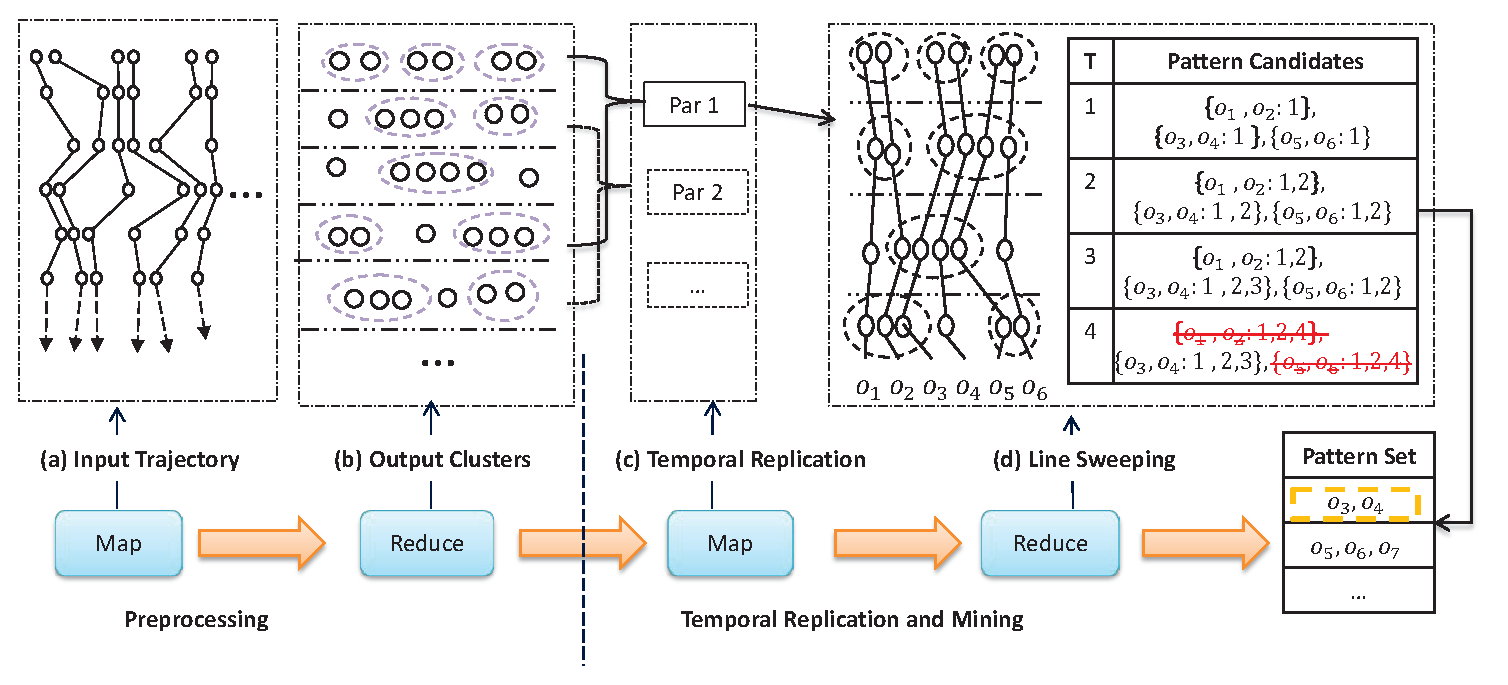
\includegraphics[width=\textwidth]{trm.eps}
\caption{Work flow of Temporal Replication and Mining. (a)(b) correspond to the first MR job which computes the clusters at each snapshot; 
(c)(d) correspond to the second MR job which uses TRM to mine GCMP in parallel.}
\label{fig:trm}
\end{figure*}

Since in the first MR job, each partition contains only one snapshot
for clustering, it is not necessary to replicate any snapshot. Thus, we
focus on describing the second MR job which is the \emph{Temporal
Replication and Mining} algorithm. We use $R$ to denote the replication factor.
The outline of TRM is 
shown in Algorithm~\ref{algo:trm_overview}.

\begin{algorithm}
\caption{Temporal Replication and Mining}
\label{algo:trm_overview}
\begin{algorithmic}[1]
\Require list of $\langle t, S_t \rangle$ pairs
\State $R \gets (\lceil \frac{K}{L} \rceil -1)*G+2K$
\State {---Map Phase---}
\label{code:trm-map-start}
\ForAll{$\langle t, S_t \rangle$}
	\ForAll{$i \in 1...R$}
		\State emit a $\langle t-i, S_t \rangle$ pair
	\EndFor  
\EndFor
\label{code:trm-map-end}
\State {---Partition and Shuffle Phase---}
\label{code:trm-par-start}
\ForAll{$\langle t, S \rangle$ pair} 
\State group-by $t$, emit a $\langle t, Par_t\rangle$
\State where $Par_t = \{S_t, S_{t+1}, .. S_{t+R}\} $
\EndFor
\label{code:trm-par-end}
\State {---Reduce Phase---}
\label{code:trm-red-start}
\ForAll{$\langle t,Par_t \rangle$}
\State lineSweepMining($Par_t$)
\label{code:trm-red-end}
\EndFor
\end{algorithmic}
\end{algorithm}

As shown in Algorithm~\ref{algo:trm_overview}, the TRM algorithm contains
three steps. First, in the map phase, each snapshot is keyed 
with its timestamp (lines~\ref{code:trm-map-start}-\ref{code:trm-map-end}). 
Second, in the partition phase, every snapshot is grouped with its next 
$R$ snapshots to form a partition (lines~\ref{code:trm-par-start}-\ref{code:trm-par-end}). 
We will shortly discuss how the $R$ value is derived. 
Third, in the reduce phase, a line sweeping method is invoked 
to mine GCMP within each partition (lines~\ref{code:trm-red-start}-\ref{code:trm-red-end}). 
It is easy to see that this method replicates a snapshots at most $R$ times.
%\subsubsection{Temporal Replication Partition}
The replication factor $R$ is critical for the performance of TRM.
If the $R$ is large, the shuffle cost as well as the reduce cost would be high. 
On the contrary, if $R$ is small, valid patterns may
be missed out. In the Algorithm~\ref{algo:trm_overview}, the 
$R$ is chosen as $(\lceil \frac{K}{L} \rceil -1)*G+2K$. We will show
later the correctness of this value.

%In the Algorithm~\ref{algo:trm_overview}, 
%the partition size is chosen as $(\lceil \frac{K}{L} \rceil -1)*G+2K$. As stated in the following
%theorem, such a partition method is sound and complete.
%\begin{theorem}[Soundness and Completeness of Replication]
%\label{thm:replication_partition}
%Let $\mathbb{P}$ be as follows: for each snapshot $S_t$, create a partition $Par_t = \{S_t, ...,S_{t+(\lceil \frac{K}{L} \rceil - 1) *G+2K}\}$. Then $\mathbb{P}$ is sound and complete.
%\end{theorem}
%\begin{proof}
%The soundness of partition can be observed from the fact that each partition represents partial trajectories with consecutive snapshots, therefore patterns in a partition can be directly mapped back to original trajectories.
%Given a valid pattern $P$, let $T' \subseteq P.T$ be the subsequence of $P.T$ which conforms to $K,L,G$ with the smallest size. Note that there could be many qualified $T'$s.  
%Let the $i^{th}$ local-consecutive part of $T'$ be $l_i$ and let the $i^{th}$ gap of $T'$ be $g_i$. Then, the size of $T'$ can be written as $\Sigma_i (l_i + g_i)$. 
%Since $T'$ conforms to $K,L,G$, then $2K \geq \Sigma_i (l_i) \geq K$, $l_i \geq L$, $g_i \leq G$. Therefore, $\Sigma_i(l_i+g_i) \leq (\lceil \frac{K}{L} \rceil -1) *G+2K$. Thus ensuring each $Par_t$ to be of that size would capture at least one of the $T'$s, therefore the pattern $P$ would be valid in $Par_t$. This proves the completeness of the partitioning method.
%\end{proof}

\subsection{Line Sweep Mining}
Each task in the reduce phase processes a partition $Par_i$, which contains
$R$ snapshots starting from snapshot $S_i$. We observe that within each $Par_i$, 
only the patterns whose object sets are contained in the first snapshot 
are necessary to be reported. Therefore, we design a simple 
\emph{line-sweep mining}(LSM) method for discovering
GCMPs. The algorithm works as in Algorithm~\ref{algo:line-sweep}.

\begin{algorithm}
\caption{Line Sweep Mining}
\label{algo:line-sweep}
\begin{algorithmic}[1]
\Require $Par_t = \{S_t, S_{t+1}, ...\}$
\State{$C \gets \{\}$} \Comment{Candidate set} \label{code:ls-can-set}
\For{$c \in S_t$} 
\label{code:ls-init-start}
\State $C$.add($\langle c, t \rangle $)
\EndFor
\label{code:ls-init-end}
\ForAll{$i \in [1,R]$}
\State $N \gets S_{t+i} \oplus C$ \label{code:ls-join}
	\ForAll {$n \in N$}
		\If{$|n.O| \geq M$}
			$C$.add($n$).
			\label{code:ls-add}
		\EndIf
	\EndFor
\State{remove unqualified candidate from $C$}
	\label{code:ls-remove}
\EndFor
\State{output qualified candidate in $C$}
\end{algorithmic}
\end{algorithm}

The algorithm scans snapshots in a partition in sequence. During the scan, it
maintains a candidate set $C$ which contains potential patterns (line~\ref{code:ls-can-set}).
The algorithm starts by inserting clusters at $S_i$ to $C$ (lines~\ref{code:ls-init-start}-\ref{code:ls-init-end}).
Subsequently, in each iteration, clusters in $C$ are joined with clusters at $S_i$ to generate
a new set of patterns $N$(lines~\ref{code:ls-join}). The valid new patterns 
form a new candidate set $C$ and any invalid patterns are discarded(lines~\ref{code:ls-add} and~\ref{code:ls-remove}).

%\begin{figure}[h]
%\centering
%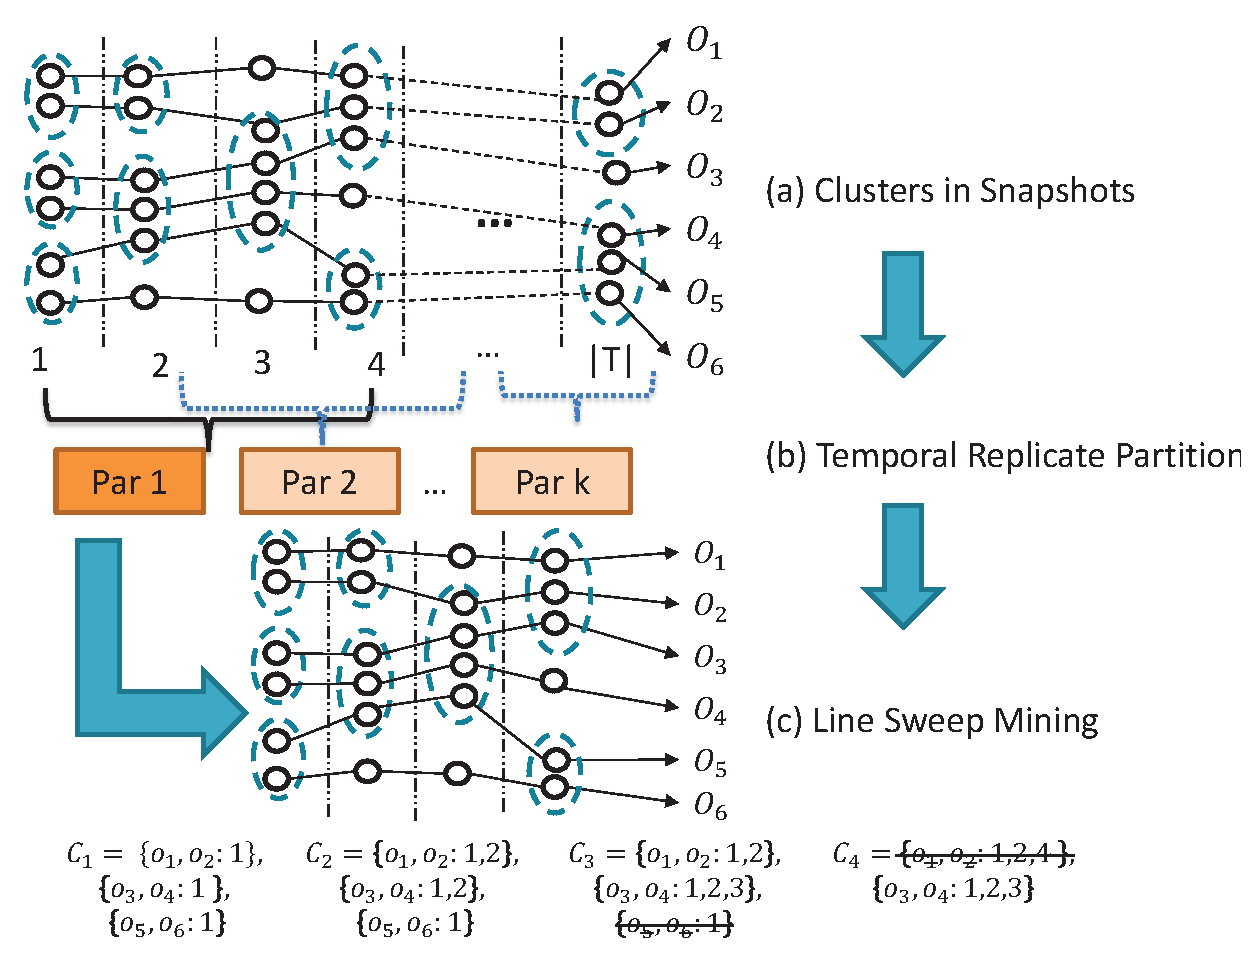
\includegraphics[width=0.5\textwidth]{trm_process.eps}
%\caption{Work flow of trajectory replication and mining}
%\label{fig:trm_process}
%\end{figure}

\subsection{Correctness of TRM}
We prove the correctness of TRM from two aspects. First,
the choice of $R = (\lceil \frac{K}{L} \rceil -1)*G+2K$ would 
not miss out any valid patterns. Second, no false patterns
are reported in any partitions. We formalize these two 
properties as \emph{completeness} and \emph{soundness} as follows:

\begin{definition}[Completeness and Soundness]
Let a partition method $\mathbb{P}$ partitions a trajectory database $Tr$ 
into segments, $Par_1,...,Par_m$. $\mathbb{P}$ is complete 
if for every valid pattern $P$ in $Tr$, $\exists Par_i$ s.t. $P$ is valid in $Par_i$. 
$\mathbb{P}$ is sound if for all patterns that are valid in any $Par_i$, they are also valid in $TR$.
\end{definition}

Apparently, in TRM, replicating the entire trajectories (i.e., $R=\mathbb{|T|}$)
meets the \emph{soundness} and \emph{completeness} requirements. However, it burdens the network shuffle and limits the parallelism. We carefully chose $R = (\lceil \frac{K}{L} \rceil -1)*G+2K$ and use
the following theorem to state the correctness:

\begin{theorem}[Correctness of Replication]
\label{thm:replication_partition}
Temporal replication partition is sound and complete.
\end{theorem}z
\begin{proof}
The soundness of partition can be observed from the fact 
that each partition represents a consecutive segments of trajectories. 
Therefore patterns in a partition can be directly mapped 
back to original trajectories. For completeness, with a
valid pattern $P$, let $T'$ be the subsequence of $P.T$ which conforms to $K,L,G$ 
with the smallest length. Note that there could be many qualified $T'$s. 
Let the $i^{th}$ local-consecutive segment of $T'$ be $l_i$ and 
let the $i^{th}$ gap of $T'$ be $g_i$. Then, the size of $T'$ can 
be written as $\Sigma_i (l_i + g_i)$.  Since $T'$ conforms to $K,L,G$, 
then $2K \geq \Sigma_i (l_i) \geq K$, $l_i \geq L$, $g_i \leq G$. 
It follows: $\Sigma_i(l_i+g_i) \leq (\lceil \frac{K}{L} \rceil -1) *G+2K$. 
If every partition is of at least such a size, then $T'$ must be
captured by at least one of the partition. Thus, the pattern $P$ would 
be valid in that partition. This proves the completeness.
\end{proof}

\begin{example}
We illustrate the entire TRM method using Figure~\ref{fig:trm} (c)(d) with $M=2, K=2, L = 2, G=2$. 
In Figure~\ref{fig:trm} (c), snapshots are combined into partitions with sizes equal to 
$(\lceil \frac{K}{L} \rceil-1) *G+2K = 4$. Then a line sweep method is performed in (d) 
for partition $1$. Each $C_i$ refers to the candidate set during sweeping snapshot $i$. 
Initially, $C_1$ contains patterns whose object set is in snapshot $1$.
As line sweeps, at snapshot $4$, since the timestamps of $\{o_1,o_2\}$ and $\{o_5,o_6\}$ 
are both $\{1,2,4\}$ which violate the $G$ constraint, 
thus the two candidates are removed from $C_4$. After all snapshots are swept, 
$\{o_3,o_4\}$ is the qualified pattern and is outputted.
\end{example}

The TRM approach though achieves good parallelism, 
it requires to replicate the data multiple times. 
Specifically, each snapshots are replicate $(\lceil \frac{K}{L} \rceil -1) *G+2K$ times. 
In the cases of \emph{swarm}, \emph{group} and \emph{platoon}, $G$ is as large as $|T|$. 
Handling those cases is equivalent to replicate the entire snapshots to each partition, 
which surrenders the benefit of parallelism.



%IMPORTANT!!!
%In contrast, it is challenging to design the second job. 
%This is because valid patterns may spray across multiple snapshots 
%or contain different object sets, where inappropriate partitioning
%of snapshots may fail to discover certain valid patterns.
%Formally, a valid partition strategy 
%needs to meet the following requirements: (a) the resulted partitions need
%to preserve enough information so that real patterns can be discovered in the reduce phase. 
%(b) the resulted partitions need to ensure that
%the patterns discovered in the reduce phase are valid patterns so that
%no further verification is required. We formalize these two 
%properties as \emph{completeness} and \emph{soundness} as follows:
%
%\begin{definition}[Completeness and Soundness]
%Let a partition method $\mathbb{P}$ partitions original trajectories $Tr$ into multiple parts, $Par_1,...,Par_m$. $\mathbb{P}$ is complete if for every pattern $P$ that is valid in $Tr$, $\exists Par_i$ s.t. $P$ is valid in $Par_i$. $\mathbb{P}$ is sound if for all patterns that are valid in any $Par_i$, they are also valid in $TR$.
%\end{definition}
%The completeness ensures that no true patterns are missed out. 
%The soundness ensures that no false patterns are reported. 
%If a partition method is both sound and complete, then it can be used
%in the second MR job to facilitate GCMP mining.
%
%Apparently, replicating the entire trajectories to each 
%partition meets the \emph{soundness} and \emph{completeness} requirements. 
%However, it burdens the network shuffle and limits the parallelism. 
%Our objective is thus to design a complete and sound partition method that minimize the network shuffles.
%In the following sections, we describe a naive \emph{temporal-based} partition-and-mining method called \emph{Temporal Replication and Mining}(TRM) towards a parallel solution of GCMP mining. Then,
%we present a novel \emph{object-based} partition-and-mining method
%called \emph{Star Partition and Mining} (SPM) which resolves
%the deficiencies of TRM method.

\section{Temporal Replication and Mining}
\label{sec:trm_solution}
The idea of \emph{Temporal Replication and Mining} (TRM)
is to group temporally closed snapshots together, such that patterns can be
mined on each group of the snapshot. In order to achieve the \emph{completeness}
and \emph{soundness} during partitioning, we allow replication of
snapshots among groups. The TRM is described in Algorithm~\ref{algo:trm_overview}.

%%The straightforward strategy of parallelizing the second stage is to vertically partition the trajectories based on snapshots. 
%A simple but effective method
%is to group neighborhood snapshots into a partition, such that every possible pattern can be mined within some of the partitions. In order to achieve the \emph{completeness},
%some of the snapshots need to be replicated on multiple executors.
%We call this method the \emph{Temporal Replication and Mining} approach. 
%The algorithm is presented as in Algorithm~\ref{algo:trm_overview}.

\begin{algorithm}
\caption{Temporal Replication and Mining}
\label{algo:trm_overview}
\begin{algorithmic}[1]
\Require list of $\langle t, S_t \rangle$ pairs
\State {---Map Phase---}
\label{code:trm-map-start}
\ForAll{$\langle t, S_t \rangle$}
	\ForAll{$i \in 1...(K-1)*G+K$}
		\State emit a $\langle t-i, S_t \rangle$ pair
	\EndFor 
\EndFor
\label{code:trm-map-end}
\State {---Partition and Shuffle Phase---}
\label{code:trm-par-start}
\ForAll{$\langle t, S \rangle$ pair} 
\State group-by $t$, emit a $\langle t, Par_t\rangle$,
\State  where $Par_t = \{S_t, S_{t+1}, .. S_{t+(\lfloor \frac{K}{L} \rfloor -1)*G+K+L}\} $
\EndFor
\label{code:trm-par-end}
\State {---Reduce Phase---}
\label{code:trm-red-start}
\ForAll{$\langle t,Par_t \rangle$}
\State lineSweepMining($Par_t$)
\label{code:trm-red-end}
\EndFor
\end{algorithmic}
\end{algorithm}

As shown in Algorithm~\ref{algo:trm_overview}, the TRM algorithm takes
three steps. First, in the map phase, each snapshot is keyed with its timestamp (lines~\ref{code:trm-map-start}-\ref{code:trm-map-end}). Second, in the partition phase, every snapshot is grouped with its next $(\lfloor \frac{K}{L} \rfloor -1)*G+K+L$ snapshots to form a partition (lines~\ref{code:trm-par-start}-\ref{code:trm-par-end}). We will shortly discuss how the group size is determined. Third, in the reduce phase, a lineSweepMining method is invoked to mine GCMP within each partition (lines~\ref{code:trm-red-start}-\ref{code:trm-red-end}). 
It is easy to see that this method replicates a snapshots at most $(\lfloor \frac{K}{L} \rfloor -1)*G+K+L$ times.

\subsubsection{Temporal Replication Partition}
The size of replication is critical for the performance of TRM algorithm.
If the size of replication is too large, the shuffle cost as well as the reduce cost would be high. 
On the contrary, if the size of replication is too small, the \emph{completeness} and \emph{soundness}
properties cannot be satisfied. In the Algorithm~\ref{algo:trm_overview}, 
the partition size is chosen as $(\lfloor \frac{K}{L} \rfloor -1)*G+K+L$. As stated in the following
theorem, such a partition method is sound and complete.
\begin{theorem}[Soundness and Completeness of Replication]
\label{thm:replication_partition}
Let $\mathbb{P}$ be as follows: for each snapshot $S_t$, create a partition $Par_t = \{S_t, ...,S_{t+(\lfloor \frac{K}{L}-1\rfloor *G+K + L )}\}$. Then $\mathbb{P}$ is sound and complete.
\end{theorem}
\begin{proof}
The soundness of partition is trivial.
Given a valid pattern $P$, let $T' \subseteq P.T$ be the subsequence of $P.T$ which conforms to $K,L,G$ with the smallest size. Note that there could be many qualified $T'$s.  
Let the $i^{th}$ local-consecutive part of $T'$ be $l_i$ and let the $i^{th}$ gap of $T'$ be $g_i$. Then, the size of $T'$ can be written as $\Sigma_i (l_i + g_i)$. 
Since $T'$ conforms to $K,L,G$, then $K+L \geq \Sigma_i (l_i) \geq K$, $l_i \geq L$, $g_i \leq G$. Therefore, $\Sigma_i(l_i+g_i) \leq \lfloor \frac{K}{L}-1\rfloor *G+K+L$. Thus ensuring each $Par_t$ to be of that size would capture at least one of the $T'$s, therefore the pattern $P$ would valid in $Par_t$. This proves the completeness of the partitioning method.
\end{proof}

\subsubsection{Line Sweep Mining}
After partition, each task in the reduce phase processes a partition $Par_i$, which contains
$\lfloor \frac{K}{L}-1 \rfloor *G+K+L$ snapshots starting from snapshot $S_i$. With such a 
partition method, we observe that within $Par_i$, only the 
patterns whose object sets are contained in the first snapshot are necessary to be reported.
Therefore, we design a simple \emph{line-sweep mining}(LSM) method for discover
GCMPs. The algorithm works as in Algorithm~\ref{algo:line-sweep}.

\begin{algorithm}
\caption{Line Sweep Mining}
\label{algo:line-sweep}
\begin{algorithmic}[1]
\Require $Par_t = \{S_t, S_{t+1}, ...\}$
\State{$C \gets \{\}$} \Comment{Candidate set} \label{code:ls-can-set}
\For{$c \in S_t$} 
\label{code:ls-init-start}
\State $C$.add($\langle c, t \rangle $)
\EndFor
\label{code:ls-init-end}
\For{$i=1; i < |Par_t|;i++$}
\State $N \gets S_i \oplus C$ \label{code:ls-join}
	\ForAll {$n \in N$}
		\If{$|n.O| \geq M$}
			$C$.add($n$).
			\label{code:ls-add}
		\EndIf
	\EndFor
\State{remove unqualified candidate from $C$}
	\label{code:ls-remove}
\EndFor
\State{output qualified candidate in $C$}
\end{algorithmic}
\end{algorithm}

The algorithm scans the snapshots in a partition in the sequential order.During the scan it
maintains a candidate set $C$ which could potentially be a valid pattern (line~\ref{code:ls-can-set}).
The algorithm starts by inserting clusters at $S_1$ to $C$ (lines~\ref{code:ls-init-start}-\ref{code:ls-init-end}).
Subsequently, in each iteration, clusters in $C$ are joined with clusters at $S_i$ to generate
a new set of patterns $N$(lines~\ref{code:ls-join}). Any valid new patterns are inserted back to $C$
and any invalid patterns are discarded(lines~\ref{code:ls-add} and~\ref{code:ls-remove}).

\begin{figure}[h]
\centering
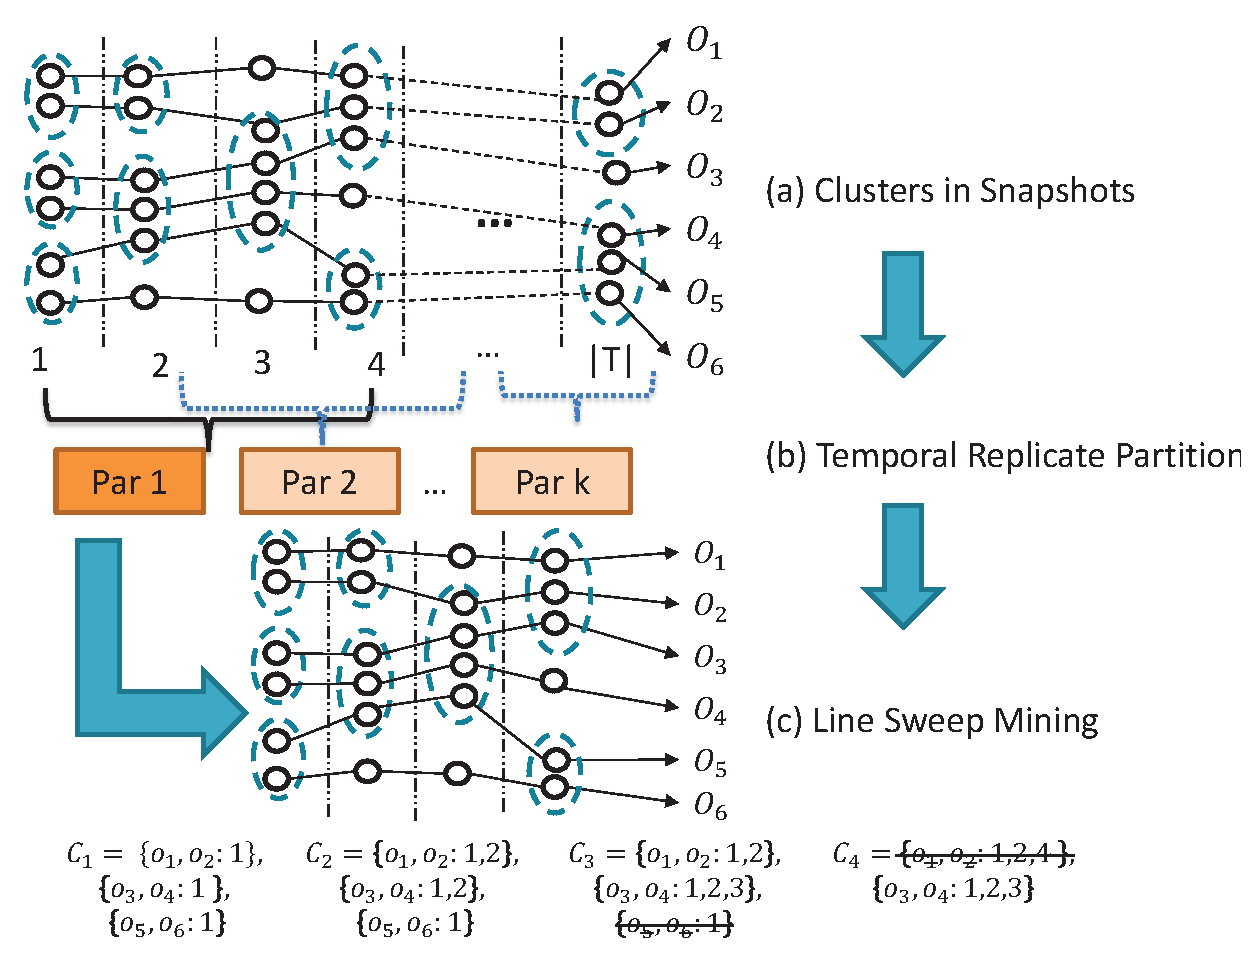
\includegraphics[width=0.5\textwidth]{trm_process.eps}
\caption{Work flow of trajectory replication and mining}
\label{fig:trm_process}
\end{figure}

\begin{example}
We illustrate the process of \emph{Trajectory Replication and Mining} in Figure~\ref{fig:trm_process} using $M=2, K=2, L = 2, G=2$. In (a), snapshots are clustered and these snapshots are the input to the TRM. Then, we compute the size 
for each partition, which equals to $\lfloor \frac{K}{L}-1 \rfloor *G+K+L = 4$. Therefore, in (b), every four snapshots
are grouped into a partition. Then a line sweep method is performed in (c) for partition 1. Each
$C_i$ refers to the candidate set  when the algorithm sweeps each snapshot. Initially, $C_1$ contains
patterns whose object set is in $S_1$. When scanning the other snapshots, patterns in $C_1$ grow
their timestamps. At $S_3$, since the timestamps of $\{o_5,o_6\}$ is $\{1,2\}$ which is neither
a qualified pattern nor matches $G$ constraint, thus this candidate is removed from $C_3$. When line
sweep finishes, only $\{o_3,o_4\}$ is the qualified pattern and is outputted.
\end{example}


The TRM approach though achieves good parallelism, 
it requires to replicate the data multiple times. 
Specifically, each snapshots are copied $\lfloor \frac{K}{L}-1 \rfloor *G+K+L$ times. 
In the cases of \emph{swarm}, \emph{group} and \emph{platoon}, $G$ is as large as $|T|$. 
Handling those cases is equivalent to replicate the entire snapshots to each partition, 
which surrenders the benefit of parallelism.


\section{Star Partition and Mining}
\label{sec:spm_solution}
TRM approach requires to replicate entire
trajectories $O(|\mathbb{T}|)$ times, which is inefficient
in parallelism. To overcome this limitation, we 
propose the \emph{Star Partition and Mining} (SPM) method.
In SPM, we design a graph model, named \emph{connection graph}, to capture 
the co-moving behavior among objects. In such a way, 
given an object $u$, all the objects potentially
co-moved with $u$ are captured in $u$'s neighborhood, which
forms a \emph{star} structure in graph terms. SPM utilizes
such structures to partition objects and then adapts an Apriori 
algorithm to discover true GCMPs from each partition.

The flow of SPM method is presented in Figure~\ref{fig:star_partition}.
SPM utilizes the same preprocessing as TRM, thus the flow starts
from clusters in each snapshot. Conceptually, the clusters 
in each snapshot forms a graph as shown in Figure~\ref{fig:star_partition} (a).
In the map phase of \emph{SPM}, a vertex together with its neighborhood 
vertexes form a star. Every star is indeed an independent partition.
Then, stars are shuffled to reducers. As in
Figure~\ref{fig:star_partition} (c), Apriori mining algorithm is adapted
to mine the GCMP patterns. The overview implementation of SPM is shown 
in Algorithm~\ref{algo:spm_overview}.

%The overview of the SPM method is presented in 
%Algorithm~\ref{algo:spm_overview}. As shown, SPM takes three phases. 
%In the map phase, objects from the same cluster form object-object pairs. 
%The object-object pairs are then paired up with the timestamp of 
%the snapshot to form a triplet(lines~\ref{code:spm-map-start}-\ref{code:spm-map-end}). 
%In the partition phase, triplets with the same leading object form a \emph{star} which will be explained shortly 
%(lines~\ref{code:spm-shuffle-start}-\ref{code:spm-shuffle-end}).
%Lastly in the reduce phase, patterns are mined from each star structure (lines~\ref{code:spm-reduce-start}-\ref{code:spm-reduce-end}).

\begin{algorithm}
\caption{Star Partition and Mining}
\label{algo:spm_overview}
\begin{algorithmic}[1]
\Require list of $\langle t, S_t \rangle$ pairs
\State {---Map phase---}
\label{code:spm-map-start}
\ForAll{$C \in S_t$}
	\ForAll {$(o_1 ,o_2) \in C \times C$}
		\If{$o_1 < o_2$}  \label{code:spm-edge-direct}
			\State emit a $\langle o_1, o_2, \{t\}\rangle$ triplet
		\EndIf
	\EndFor
\EndFor
\label{code:spm-map-end}

\State {---Partition and Shuffle phase---}
\label{code:spm-shuffle-start}
\ForAll{$\langle o_1, o_2, \{t\}\rangle$ triplets} 
	\State group-by $o_1$, emit $\langle o_1, Sr_{o_1} \rangle$ 
	%\State group-by $o_2$, emit $\langle o_2, Sr_{o_2} \rangle$
\EndFor
\label{code:spm-shuffle-end}

\State {---Reduce phase---}
\label{code:spm-reduce-start}
\ForAll{$\langle o, Sr_{o} \rangle$}
\State Apriori($Sr_o$)
\EndFor
\label{code:spm-reduce-end}

\end{algorithmic}
\end{algorithm}

\subsection{Star Partition}
The intuition of the star partition is that, if two objects are part 
of the same pattern, they must belong to the same cluster at 
those snapshots. Therefore, we may link objects that belong to 
the same cluster to form the \emph{connection graph}. Objects that are
not connected surely fail to form a pattern. We may then
partition the connection graph based on vertex connectivity
such that mining GCMPs can be done in parallel. 
We formally define the \emph{connection graph} as follows:
\begin{definition}[Connection Graph]
A connection graph is an undirected graph $G=(V:E)$, where 
each $v \in V$ represents an object. An edge $e(s,t)= ET \in E$ 
contains the timestamp sequence at which $s,t$ are in the same cluster,
i.e., $\forall t \in ET, C_t(s) = C_t(t)$. 
\end{definition}

In graph theory, a \emph{star} of a vertex $u$ is the
the set of neighborhood vertexes of $u$. To utilize \emph{star}
partition, since a vertex may appear in multiple stars, 
some replications of vertexes are required. In order to avoid replication 
of edges, we use the \emph{directed star} as follows:

\begin{definition}[Directed Star]
Assign each vertex in $G$ an ID, a direct star of a vertex $s$, denoted as $Sr_s$, 
is the set of incidental edges on $s$
such that $\forall e(s,t) \in Sr_s$, $s < t$. We name $s$
as the \emph{central vertex} of $Sr_s$.
\end{definition}

By leveraging the \emph{directed star}, we avoids replicating the edges. 
A \emph{Connection graph} and \emph{star} examples are 
shown in Figure~\ref{fig:star_partition} (a) and (b). In (a), a connection graph is formed
based on the example in Figure~\ref{fig:related_work}.
In (b), 5 stars are presented. It can be figured out that by leveraging directed star, 
no edges are replicated. In implementation,
as show in Algorithm~\ref{algo:spm_overview} line~\ref{code:spm-edge-direct}, the
comparison between vertices/objects are based on the vertex/object IDs.

\begin{figure*}[t]
\centering
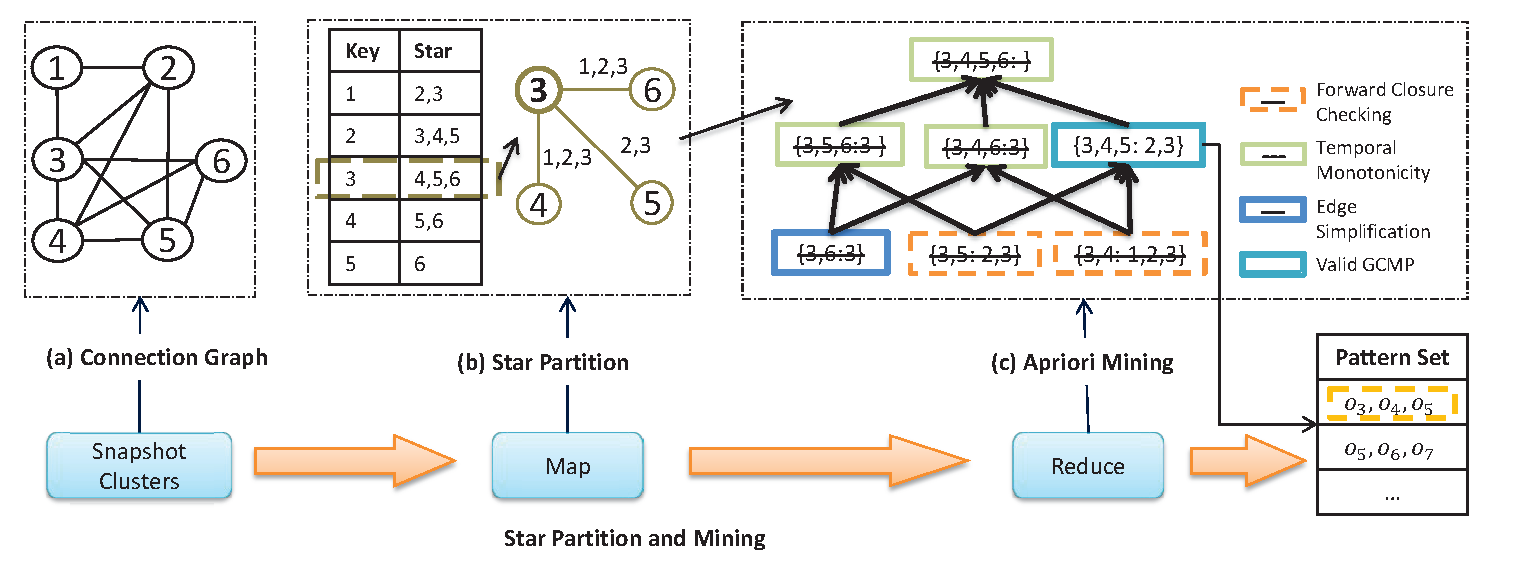
\includegraphics[width=0.9\textwidth]{spm.eps}
\caption{Star partition and mining. (a) Conceptual connection graph from Figure 1.(b) Five star partitions are generated
(c) Apriori Mining with various pruning techniques.}
\label{fig:star_partition}
\end{figure*}

%After computing the star, each partition is applied with a reduce task. 
%Indeed, a star $Sr_s$ can be viewed as a subset of original trajectories. 
%This is done by treating each vertex in $Sr_s$ as an object. 
%The time sequence of $s$ is the union of all edges in $Sr_s$. 
%And the time sequence of $v \neq s$ is the edge $(s,v)$. Therefore, we
%are able to mine stars from the similar trajectory concepts.

\subsection{Apriori Mining}
To systematically discover valid patterns in each star, 
we design the \emph{Apriori Mining} algorithm. 
To describe the  algorithm, we call a candidate pattern $R$-pattern 
if the size of its object set is $R$.  Therefore, each edge
in the star is effectively a $2$-pattern. The intuition of Apriori mining
is the observation that $(R+1)$-patterns can be generated
from $R$-patterns and $2$ patterns. Thus, we may iteratively 
enumerate pattern candidates with all possible sizes.
In particular, initially, for each $e(s,v)=ET$, pattern $p=(\{s,v\}, ET)$ is formed. 
During each iteration, we generate $(R+1)$-patterns by joining $R$-patterns 
with the $2$-patterns. Technically, the join between $p_1=(O_1:T_1)$ and $p_2=(O_2:T_2)$
generates a new pattern $p_3=(O_1 \cup O_2:T_1 \cap T_2)$. Note that in $Sr_s$,
each $R$-pattern contains the object $s$, thus the join only 
grow a $R$-pattern at most to a $(R+1)$-pattern.
Our mining algorithm stops where no further patterns are generated. 
The algorithm is illustrated as in Algorithm~\ref{algo:apriori_mining}.

\begin{algorithm}
\caption{Apriori Mining}
\label{algo:apriori_mining}
\begin{algorithmic}[1]
\Require{$Sr_s$}
\State { Lv $\gets \{\}$,Ground $\gets \{\}$, Output $\gets \{\}$}
\ForAll{$e(s,t) = T \in Sr_s$}
\State Ground.add($\langle \{s,t\}, T \rangle$);
\State Lv $\gets$ Ground;
\EndFor
\While{true}
	\If{Lv is not empty} 
		\State{LvCand $\gets \{\}$ }
		\ForAll{$cand_v \in Lv$}
			\ForAll{$cand \in $Ground}
				\State $p \gets cand_v$ join $cand$
				\If{$p.T$ is a candidate sequence} 
					\State LvCand.add($p$)
				\EndIf
			\EndFor
		\EndFor
		\If{$Lv$ is a pattern}
			\State{Output.add($Lv$)}
			\State{break}			 
		\EndIf
		\State {Lv $\gets$ LvCand}
	\Else
		\State{break}
	\EndIf
\EndWhile
\State output.addAll($Lv$)
\State \Return output
\end{algorithmic}
\end{algorithm}
 
An illustration of Algorithm~\ref{algo:apriori_mining} is shown in Figure~\ref{fig:star_partition} (c).
As shown, the star $Sr_3=\{3,4,5,6\}$ initially generate three $2$-candidates. At every iteration, 
higher level candidates are generated by joining lower level candidates. When no more candidates 
can be generated, the algorithm stops by outputting the valid patterns.

It is notable that, in star partition, original data is 
replicated for $O(|\mathbb{O}|)$ times as each object may 
be sent to $O(|\mathbb{O}|)$ stars. Since in reality, $|\mathbb{T}| \gg |\mathbb{O}|$, 
the star partition is more scalable than the temporal replication.
In later sections, we will describe several engineering level optimization to further reduce the amount of replicated data.
%It is notable that Algorithm~\ref{algo:apriori_mining} takes exponential
%time to mine GCMP. There are two major factors dragging 
%down the performance. First, the size of $Sr_s$ affects the initial 
%size of $2$-patterns. Second, the candidates generated in each 
%level affects the join performance. In later
%sections, we exploit some properties of GCMP to reduce the two factors.

\subsection{Analysis of SPM}
The analysis of SPM contains two parts. We first prove the correctness
of SPM. Then, we analyze the work load distribution of the star sizes.

\subsubsection{Correctness}
Although star partition is performed based on the connection graph, 
each star is indeed a projection of original trajectories.
To see this, each vertex can be viewed as an object. 
The timestamps of center vertex $s$ is the union of all the 
edges in $Sr_s$. The timestamps of vertex $v \neq s$ is the 
edge $e(s,v)$. Therefore, stars can be viewed as a trajectory
database, where GCMP can be similarly defined. Using the same 
notions as Definition 4, we state the correctness
of star partition as follows:

\begin{theorem}[Soundness and Completeness of Star Partition]
Star partition is sound and complete.
\end{theorem}

\begin{proof}
For the soundness,
if $P$ is a valid pattern in $Sr_s$, then at every time $t$, 
$\forall o_1, o_2 \in P.O$, $C_t(o_1) = C_t(o_2)$.
By definition, $P$ is valid in the original trajectories.
For the completeness,
if $P$ is a valid pattern in original trajectories, 
let $s$ be the object with smallest ID in $P.O$. 
Based on the definition of GCMP, $\forall t \in P.T$, $\forall o \in P.O$, $C_t(s) = C_t(o)$.
It follows that all object $o \in P.O$ are in $Sr_s$. 
Furthermore, every timestamp in $P.T$ is included
in $Sr_s$. Therefore, $P$ is a valid pattern in $Sr_s$.
\end{proof}


\subsubsection{Optimal Star Partition}
An important concern in design parallel algorithms is 
the distribution of work loads. Unlike TRM where each partition
contains equal-sized snapshot, the size distribution 
of stars remains SPM unknown. 
Traditionally, the quality of a partition strategy 
is measured based on two aspects: (1) the number of result partition, which
affects the maximum parallelism
(2) the balance of partition sizes, which affects the finishing
time of a job. We notice that, in star partition, the total sizes of 
stars are invariant. Therefore, the quality of a partition strategy
can be formalized as the \emph{skewness}, which is the maximum star size
among all stars. Smaller \emph{skewness} naturally results in more partitions
and less imbalance.


\begin{figure}[h]
\centering
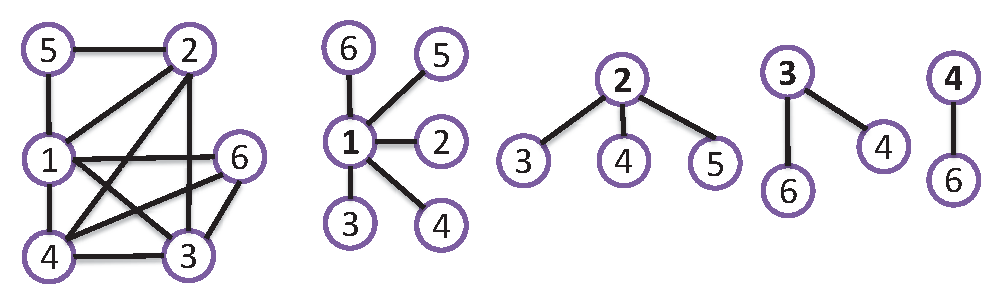
\includegraphics[width=0.4\textwidth]{star-alt.eps}
\caption{An alternative numbering and partitioning of the connection graph in Figure~\ref{fig:star_partition}.}
\label{fig:star-alt}
\end{figure}

Interestingly, we note that the \emph{skewness} of star partition is affected by
the way the vertexes are numbered in the connection graph. For example,
Figure~\ref{fig:star-alt} gives two valid numbering of vertexes 
in the same connection graph, but produces two different set of stars. 
The upper partitioning constructs four stars with the maximum star consisting of 5 edges.
The lower partitioning constructs five stars with the maximum star consisting of 3 edges.
Apparently the upper partitioning is inferior because its \emph{skewness} is 5 while the
lower one's \emph{skewness} is 3.

Ideally we wish to find a numbering scheme of connection graph
that minimize the \emph{skewness}.
To quantify the objective, we design an linear algebra model as follows: Let $G$ denote a connection graph.
Let $\mathbb{A}$ be an arbitrary numbering of vertexes in $G$.
Let $(A:a_{i,j})$ be a boolean assignment matrix wrt. $\mathbb{A}$ (i.e., $a_{i,j}$ indicates whether vertex $j$ is included in $Sr_i$). Let vector $\vec{b}$
be the \textit{one}\footnote{Every element in $\vec{b}$ is $1$} vector. Let $\vec{c} = A\vec{b}$, then
each $c_i \in \vec{c}$ denotes the size of star for vertex $i$.
Therefore, minimizing the \emph{skewness} can be formulated as follows:
\begin{equation}
\mathbb{A}  = \argmin(||A\vec{b}||_\infty) \text{,where } ||A\vec{b}||_\infty = \max_{1\leq j \leq n}(c_j)
\end{equation}

It is challenging to directly optimize the above equation. 
First, suppose there are $n$ vertexes in $G$, enumerating
all possible $\mathbb{A}$s leads to $n!$ combinations. 
Such a high complexity is trivially unpractical. Second,
since $G$ is only conceptual at runtime, 
the load planning cannot be done beforehand. 
Despite these challenges, we observe that there is a 
$O(1)$ time solution which is good enough as stated in the 
following theorem.

\begin{theorem}[Balance of Star Partition]
Let $G$ be a connection graph with $n$ vertexes and the average degree $d$.
Let $\mathbb{A}^*$ be the optimal numbering wrt. Equation 1.
For any numbering, $\mathbb{A}$, with high probability, the 
absolute skewness difference between $\mathbb{A}^*$ and $\mathbb{A}$ is $O(\sqrt{n \log n})$.
That is, it is very likely that 
$||\mathbb{A}\vec{b}||_\infty = ||\mathbb{A}^*\vec{b}||_\infty + O(\sqrt{n \log n})$.
\end{theorem}

\begin{proof}
Let $\mathbb{A}^*$ be the optimal solution wrt Equation 1. Since we have a star
for each object, by the degree-sum formula and pigeon-hole theorem, $||A^*\vec{b}||_\infty \geq d/2$.
Next, let $e_{i,j}$ be an entry in the adjacent matrix of $G$. Note that edges in $G$ are independent. 
Let $d_i$ denote the degree of vertex $i$ in $G$. 
It follows that $E[d_i]=E[\Sigma_{1\leq j \leq n}e_{i,j}]=d$.
Since in the star partition, each edge is assigned to the vertex
with smaller IDs, the connection between $a_{i,j}$ and $e_{i,j}$ can be written as:
\begin{equation*}
a_{i,j} = \begin{cases}
			e_{i,j}, i>j \\
			0, otherwise
		  \end{cases}  
\end{equation*}
There are two observations made on the above equation. First, since $e_{i,j}$s are independent,
$a_{i,j}$s are independent. Second, since $i>j$ and $e_{i,j}$ are independent. 
$E[a_{i,j}] = E[e_{i,j}]E[i>j]= E[e_{i,j}]/2$.

By definition, $c_i = \Sigma_{1\leq j \leq n} a_{i,j}$, 
is a sum of $n$ independent 0-1 variables. Taking expectation on both sides, 
we get: $E[c_i] = E[\Sigma_{1\leq j \leq n} a_{i,j}]=E[\Sigma_{1\leq j \leq n} e_{i,j}]/2 = d/2$. Let $\mu =E[c_i] = d/2$, 
$t = \sqrt{n\log n}$, by Hoeffding's Inequality, the following holds:
\begin{equation*}
\begin{split}
	Pr(c_i \geq \mu + t) 
						&\leq \exp(\frac{-2t^2}{n}) \\
						&= \exp(-2\log n) = n^{-2}
\end{split}
\end{equation*}

The first step is due to the fact that all $a_{i,j}$ are bounded in the range of [0,1]. 
Next, since the event $(\max_{1\leq j \leq n}(c_j) \geq \mu + t)$ can be viewed as
$\cup_{c_i} (c_i \geq \mu + t )$, by Union Bound, we achieve the following:
\begin{equation*}
\begin{split}
	Pr(||A\vec{b}||_\infty \geq \mu + t) &=Pr(\max_{1\leq j \leq n}(c_j) \geq \mu + t)  \\
		& = Pr(\cup_{c_i} (c_i \geq \mu + t )) \\
		&\leq \Sigma_{1 \leq i \leq n} Pr(c_i \geq \mu + t) \\
		& = n^{-1} = 1/n
\end{split}
\end{equation*}
Substitute $t$ and $\mu$, we achieve the following concise form:
\begin{equation*}
	Pr(||A\vec{b}||_\infty \geq (d/2 + \sqrt{n\log n})) \leq 1/n
\end{equation*}
This indicates that, the probability of $(||A\vec{b}||_\infty-d/2)$ being less than or equal to $ O(\sqrt{n\log n})$ is $(1-1/n)$. With the observed fact that $||A^*\vec{b}||_\infty \geq d/2$, we conclude that
with probability greater than $(1-1/n)$, 
the difference between $||A\vec{b}||_\infty$ and $||A^*\vec{b}||_\infty$ is less than $O(\sqrt{n\log n})$.
\end{proof}

In fact, we have a tighter bound of $||A\vec{b}||_\infty -||A^*\vec{b}||_\infty$ if 
the connection graph is \emph{dense}. Specifically, if $d\geq \sqrt{12\log n}$, the following
equation holds:
\begin{equation*}
Pr(||A\vec{b}||_\infty \geq (d/2 + O(\sqrt{d\log n})) \leq 1/n
\end{equation*}

\section{Optimization}
\label{sec:optimization}
In this section, we describe several optimizations to the star-partition and mining algorithm.
In addition, we also address some practical issues when deploying the SPM algorithm
to real MapReduce based systems.

%We have analyzed that the bottlenecks of Algorithm~\ref{algo:apriori_mining} 
%lies in two factors. The size of each $Sr_s$ and the size of candidates in each level of Apriori.
%In this section, we provide several optimizations to boost the bottlenecks.
%\subsection{Edge Reduction by Direction}
%The first spot for reducing the size of $Sr_s$ is to remove the replicated edges. As shown in Algorithm~\ref{algo:spm_overview}, each edge in the conceptual graph is replicated twice in generating the star-structure. The purpose of replication is to ensure the completeness of star partition. However, this replication can be avoided if we choose an appropriate way of partitioning. 
%
%We design the edge partitioning method by edge direction. Instead of building a conceptual graph that is undirected, we create the directed conceptual graph as follows: First, we assign each object a unique number. Then
%for a cluster $C_t$ in snapshot $S_t$, for any pair $(u,v) \in C_t$, an edge $e(u,v) = \{t\}$ is created if $u < v$. It is easy to see that the directed conceptual graph is a DAG. We then create each $Sr_u$ by including all the outgoing edges of $u$. By so doing, each edge is assigned to only one star, thus avoids the replications. We use the following theorem to ensure the completeness of the edge direction method.
%
%\begin{theorem}[Sound and Completeness of Edge Direction]
%Star partition with edge direction is sound and complete.
%\end{theorem}
%\begin{proof}
%It is notable that each star is a subset of original trajectories, thus the soundness is trivially true. For completeness, if $P$ is valid pattern, then let $s$ be the object of the smallest number in $P.O$, i.e., $s=\min_{o \in P.O}(o)$. Since $s$ is smallest and the all other objects in $P.O$ is connected with $s$. Therefore, $P.O \equiv Sr_s$, which indicates that $P.O$ is also a pattern in $Sr_s$.
%\end{proof}
%An example of edge direction is shown in Figure~\ref{fig:star_partition}. As shown,
%by adapting the direction method, half the size of $S_r$'s is reduced. This clearly brings efficiency in both shuffling and apriori mining.

\subsection{Edge Simplification}
Each edge $e(s,v)$ in $Sr_s$ contains a time sequence $ET$ 
which represents the co-occurrence of $s$ and $v$. We notice that the edge 
between $s$ and $t$ is not always necessary. For example, if an edge has a
cardinality less than $K$, it is unnecessary to include this edge to 
$Sr_s$ since it cannot contribute to any patterns.
This motivates us to simplify the edges in $Sr_s$ 
to boost the overall performance.

Our goal of edge simplification is to, given a time sequence $T$, find a subsequence
of $T' \subseteq T$, such that $T'$ is potentially conforms to $K,L,G$. And we
wish $|T'|$ to be as small as possible.  
We star-off by observing that for every time sequence $T$, $T$ can be 
divided into a set of maximally $G$-connected subsequences. Note that
a maximally $G$-connected subsequence can potentially contribute to
a pattern if it conforms to $K,L$.
Therefore, we are able to reduce $T$
to its maximally $G$-connected subseuqnces which conform to $K,L$.

To formally describe the idea, we define the a \emph{candidate sequence} as follows:

%\begin{definition}[Candidate Sequence]
%Given the pattern parameters: $K,L,G$, a sequence $T$ is 
%a \emph{partly candidate} sequence if exists one of its maximal $G$-connected
%subsequence $T'$ such that $T'$ confirms to $L,K$.
%\end{definition}

%For example, let $L = 2, K = 4, G = 2$, sequence $T_1=(1,2,4,5,6,9,10,11)$ 
%is a \emph{partly candidate sequence} since $T_1[1:5] = (1,2,4,5,6)$ is a valid
%pattern wrt. $L,K,G$. In contrast, $T_2=(1,2,5,6,7)$ is not a valid partly candidate sequence.
%
%Observing that only partly candidate sequence can be potentially contribute to a 
%pattern. Therefore, given an edge $e(s,t)=T \in Sr_s$, if $T$ is not a partly
%candidate sequence, it can be pruned from $Sr_s$. To efficiently
%test whether a given sequence is partly candidate, we define the \emph{Fully Candidate Sequence}:

\begin{definition}[Candidate Sequence]
Given the pattern parameters: $L,K,G$, a sequence $T$ is a \emph{Candidate Sequence} 
if for any of its maximal $G$-connected sequence $T'$, $T'$ conforms to $L,K$.
\end{definition}

For example, let $L = 2, K = 4, G = 2$, sequence $T_1=(1,2,4,5,6,9,10,11,13)$ is 
not a fully candidate sequence since one of its maximal $G$-connected sequence $(9,10,11)$
is not a partly candidate sequence. In contrast, sequence $T_2=(1,2,4,5,6)$ is 
a fully candidate sequence.

To reduce a sequence $T$ to a candidate sequence, we need to strip out its 
maximal $G$-connected subsequences which does not form to $K,L$. Such a reduction
takes two rounds scan of $T$ as shown in Algorithm~\ref{algo:simp_prune}. In the 
first round, the consecutive portions of $T$ with size less than $L$ are removed.
In the second round, the maximal $G$-connected sequences of size less than $K$ are
removed. Clearly the simplification algorithm runs in $O(|T|)$ time.
\begin{algorithm}
\caption{Edge Simplification}
\label{algo:simp_prune}
\begin{algorithmic}[1]
\Require $T$
\State{---Remove the consecutive portion with size less than $L$---}
\State $c \gets 0$
\For {$i \in (0,...,|T|)$}
	\If{$T[i] - T[i-1] != 1$} 
		\If{$i - c < L$} 
			\State $T$ remove $[c:i)$
		\EndIf
		\State $c \gets i$
	\EndIf
\EndFor
\State{---Remove the pseduo-consecutive portion with size less than $K$---}
\State $s\gets 1$, $c\gets 0$
\For{$i \in (0: |T|)$}
	\If{$T[i] - T[i-1] > G$}
		\If{$s < K$}   
			\State $T$ remove $[c:i)$
		\EndIf
		\State {$c \gets i$, $s \gets 1$}
	\Else
		\State $s++$
	\EndIf
\EndFor
\end{algorithmic}
\end{algorithm}

\begin{example}
Take $T_1=\{1,2,4,5,6,9,10,11,13\}$ as an example of edge simplification. Let $L = 2, K = 4, G = 2$.
In the first round of scan. $T_1$ reduces to $\{1,2,4,5,6,9,10,11\}$. The consecutive subsequence $\{13\}$
is removed by $L=2$. $T_1$ has two maximal $G$-consecutive subsequences, which 
are $\{1,2,4,5,6\}$ and $\{9,10,11\}$. Since $K=4$, $\{9,10,11\}$ is removed
from $T_1$ in the second round of scan. Therefore, $T_1$ is simplified to $\{1,2,4,5,6\}$.
\end{example}

%
%Based on the fully candidate sequence, we can reduce an sequence $T$ to a 
%fully candidate sequence by striping out its non-partly candidate maximal pseudo-consecutive 
%sequences. The reduction works as in Algorithm~\ref{algo:simp_prune}. It takes two
%rounds of scan of an input $T$. In the first round of scan,
%the consecutive portion of $T$ with size less than $L$ is removed.
%In the second round of scan, the pseudo-consecutive portion of $T$ with size less than $K$
%is removed. 


By leveraging the edge simplification technique, 
the size of the edges in $Sr_s$ can be greatly reduced. If
an edge cannot be reduced to a candidate sequence, then it is directly removed from $Sr_s$.
If an edge can be reduced to a candidate sequence, replacing itself 
by the candidate sequence results in a more compact storage.

%We use the following theorem to state the completeness and correctness of the 
%edge reduction algorithm.
%\begin{theorem}[Soundness and Completeness Edge Simplification]
%Star partition with edge simplification is sound and complete.
%\end{theorem}
%
%\begin{proof}
%Soundness of the star partition is not affected by edge simplification since each star is a subset of original trajectory. For completeness, notice that given a time sequence $T$, and any of its maximal $G$-connected subsequence $T'$, if $T'$ does not conform to $L,K$, then $T'$ cannot contribute to any patterns. 
%\end{proof}


\subsection{Candidate Pruning}
\subsubsection{Temporal monotonicity}
During the apriori phase, we repeatedly join candidate patterns in different levels to generate a larger set
of a patterns. We observe that traditional monotonic property of Apriori algorithms \textbf{does not}
hold in GCMP mining. That is given two candidate $P_1, P_2$, if $P_1.O \subset P_2.O$ and $P_1$ is not 
a valid pattern, then $P_2$ may or may not be a valid pattern. However, we notice that
we may form another monotonic property based on the \emph{candidate sequence} such that
the Apriori algorithm could still benefit.

The intuition is that if a candidate $P_1.T$ cannot be reduce to a \emph{candidate sequence}, then $P_1$ cannot 
be valid pattern. Furthermore, any candidate $P_2$, with $P_1.O \subset P_2.O$ cannot be a valid pattern.
This \emph{temporal monotonic property} 
is explicitly described as in the follow theorem:

\begin{theorem}[Temporal Monotonic Property of GCMP]
Given the temporal parameters $L,G,K$, for a candidate $c$ in Algorithm~\ref{algo:apriori_mining},
if $c.T$ cannot be reduced to a candidate sequence, then for any candidate $c'$ with $c.O \subset c'.O$, $c'$ can be pruned.
\end{theorem}
\begin{proof}
Let $c_1$, $c_2$ be two candidates with $c_1.O \subset c_2.O$. It is easy to see that $c_1.T \supseteq c_2.T$.
If $c_1.T$ cannot be reduced to a candidate sequence, then any subset of $c_1.T$ cannot
be reduced. It follows that $c_2.T$ cannot be reduced neither. Thus,
if $c_1.T$ cannot be reduced to a candidate sequence, $c_2$ can be pruned. 
\end{proof}

\subsubsection{Forward closure checking}

\begin{example}
We use Figure~\ref{fig:star_partition} (c) to demonstrate the candidate pruning. As shown, at the initial stage, $\{3,6:1,4\}$ is pruned, since $\{1,4\}$ is not a candidate sequence. By temporal monotonicity, candidates containing objects $\{3,6\}$ can all be pruned. Therefore, we are able to directly prune $\{3,4,6\}$, $\{3,5,6\}$ and $\{3,4,5,6\}$.
\end{example}
%
%With the help of the \emph{Monotonic Property}, the number of new candidates in each level is greatly reduced. We verify this in the experiment session as well.
\subsection{Load Balancing}

\subsection{Duplication Detection}

\subsection{Handling Overlapping Clusters}
\input{sec8_experiment}
\input{sec9_conclusion}

% The following two commands are all you need in the
% initial runs of your .tex file to
% produce the bibliography for the citations in your paper.
\bibliographystyle{IEEEtr}
\small
\bibliography{citations}
\end{document}
